\documentclass{sig-alternate}
%%%%%%%%%%%%%%%%%%%%%%%%%%%%%%%%%%%%%%%%%%%%%%%%%%%%%
% The following lines are needed to make sure that
% algorithm2e works with sig-alternate and others.
%%%%%%%%%%%%%%%%%%%%%%%%%%%%%%%%%%%%%%%%%%%%%%%%%%%%%

\usepackage[ruled,vlined,linesnumbered]{algorithm2e}
\usepackage{amsmath,amssymb}
\usepackage{epsfig}
\usepackage{color}
\usepackage{url}
\usepackage{varioref}
%\usepackage[all=normal,bibbreaks=tight, mathspacing=tight]{savetrees}
\newcommand{\subparagraph}{} %introduced for titlesec package
\usepackage[compact]{titlesec} %for squeezing. refer titlespacing in squeeze
\usepackage{setspace} %for reducing the space in bibliography
\usepackage{pifont} %for the markers on the author's affiliation
\usepackage[font=bf]{caption}

%\makeatletter
%\let\@copyrightspace\relax
%\makeatother

\newcommand{\theoremname}{Theorem}
\newcounter{thm}
\newenvironment{thm}{%
  \par\medskip\refstepcounter{thm}%
  \noindent\textbf{Theorem \thethm:}\quad}{\par\medskip}
\labelformat{thm}{\theoremname~#1}

\newcommand{\definitionname}{Definition}
\newcounter{defn}
\newenvironment{defn}{%
  \par\medskip\refstepcounter{defn}%
  \noindent\textbf{Definition \thedefn:}\quad}{\par\medskip}
\labelformat{defn}{\definitionname~#1}

\newcommand{\lemmaname}{Lemma}
\newcounter{lemma}
\newenvironment{lemma}{%
  \par\medskip\refstepcounter{lemma}%
  \noindent\textbf{Lemma \thelemma:}\quad}{\par\medskip}
\labelformat{lemma}{\lemmaname~#1}

\newcommand{\corollaryname}{Corollary}
\newcounter{corollary}
\newenvironment{corollary}{%
  \par\medskip\refstepcounter{corollary}%
  \noindent\textbf{Corollary \thecorollary:}\quad}{\par\medskip}
\labelformat{corollary}{\corollaryname~#1}


\DeclareMathOperator*{\argmin}{arg\,min}

\def\Set#1{{\left\{\,#1\,\right\}}}
\def\norm#1{{\left\|\,#1\,\right\|}}
\def\abs#1{{\left|\,#1\,\right|}}
\def\divv{\mathop{\rm div}\nolimits}
\def\dist{\mathop{\rm dist}\nolimits}
\def\diam{\mathop{\rm diam}\nolimits}
\def\Proj{\mathop{\rm Proj}\nolimits}
\def\norm #1{\|#1\|}
\def\abs #1{|#1|}
\def\argmax{\mathop{\rm arg\,max}}
\def\argmin{\mathop{\rm arg\,min}}
\def\define{:=}
\def\inprod#1#2{\langle #1,\,#2\rangle}
\def\W{{\cal W}}
\def\sgn{{\rm sgn}}


\newcommand{\algofull}[0]{{Text Outliers using Nonnegative Matrix Factorization}}
\newcommand{\algo}[0]{{TONMF}}
\newcommand{\red}[1]{\begin{color}{red}#1\end{color}}

\newcommand{\charu}[1]{{\color{cyan}{\bf\sf [New Charu: #1]}}}
%\newcommand{\ramki}[1]{{\color{red}{\bf\sf [New Ramki: #1]}}}
\newcommand{\ramki}[1]{#1}
\newcommand{\woo}[1]{{\color{green}{\bf\sf [New Woo: #1]}}}

%customize savetrees
%\makeatletter
%\@st@tight@bibliographyfalse
%\makeatother

%\input{squeeze}

\begin{document}

\title{Outlier Detection for Text Data : An Extended Version}

\numberofauthors{4}
%
%\author{
%\alignauthor Ramakrishnan Kannan \textsuperscript{\ddag}\\
%%\affaddr{Georgia Institute of Technology}\\
%%\affaddr{Atlanta, GA, USA}\\
%\email{rkannan@gatech.edu}
%%
%\alignauthor Hyenkyun Woo \textsuperscript{\ding{169}}\\
%%\affaddr{Korea Institute for Advanced Study}\\
%%\affaddr{Seoul, Korea}\\
%\email{hyenkyun@kias.re.kr}
%%
%\alignauthor Charu C. Aggarwal \textsuperscript{\ding{86}}\\
%%\affaddr{IBM T. J. Watson Research Center}\\
%%\affaddr{Hawthorne, NY, USA}\\
%\email{charu@us.ibm.com}
%%
%%\and
%\alignauthor Haesun Park\textsuperscript{\ddag}\\
%%\affaddr{Georgia Institute of Technology}\\
%%\affaddr{Atlanta, GA, USA}\\
%\email{hpark@cc.gatech.edu}
%\end{tabular}\newline\begin{tabular}{c}
%\affaddr{\textsuperscript{\ddag}Georgia Institute of Technology,Atlanta, GA, USA}\\
%\affaddr{\textsuperscript{\ding{169}}Korea Institute for Advanced Study, Seoul, Korea}\\
%\affaddr{\textsuperscript{\ding{86}}IBM T. J. Watson Research Center, Hawthorne, NY, USA}\\
%}

\author{
\alignauthor Ramakrishnan Kannan\\
\affaddr{Oak Ridge National Laboratory}\\
\affaddr{Oak Ridge, TN, USA}\\
\email{kannanr@ornl.gov}
%%
\alignauthor Hyenkyun Woo \\
\affaddr{Korea University of Technology and Education}\\
\affaddr{Republic of Korea}\\
\email{hyenkyun@koreatech.ac.kr}
%%
\alignauthor Charu C. Aggarwal\\
\affaddr{IBM T. J. Watson Research Center}\\
\affaddr{Yorktown Heights, NY, USA}\\
\email{charu@us.ibm.com}
%%
\and
\alignauthor Haesun Park\\
\affaddr{Georgia Institute of Technology}\\
\affaddr{Atlanta, GA, USA}\\
\email{hpark@cc.gatech.edu}
}

\maketitle

\begin{abstract}
%Although Deep Convolutional Neural Networks (CNNs) have liberated their power in various computer vision tasks, the most important components of CNN, convolutional layers and fully connected layers, are still limited to linear transformations. In this paper, we propose a novel Factorized Bilinear (FB) layer to model the pairwise feature interactions by considering the quadratic terms in the transformations. Compared with existing methods that tried to incorporate complex non-linearity structures into CNNs, the factorized parameterization makes our FB layer only require a linear increase of parameters and affordable computational cost. To further reduce the risk of overfitting of the FB layer, a specific remedy called DropFactor is devised during the training process. We also analyze the connection between FB layer and some existing models, and show FB layer is a generalization to them. Finally, we validate the effectiveness of FB layer on several widely adopted datasets including CIFAR-10, CIFAR-100 and ImageNet, and demonstrate superior results compared with various state-of-the-art deep models.

Neural Style Transfer~\cite{neuralart} has recently demonstrated very exciting results which catches eyes in both academia and industry. Despite the amazing results, the principle of neural style transfer, especially why the Gram matrices could represent style remains unclear. In this paper, we propose a novel interpretation of neural style transfer by treating it as a domain adaptation problem. Specifically, we theoretically show that matching the Gram matrices of feature maps is equivalent to minimize the Maximum Mean Discrepancy (MMD) with the second order polynomial kernel. Thus, we argue that the essence of neural style transfer is to match the feature distributions between the style images and the generated images. To further support our standpoint, we experiment with several other distribution alignment methods, and achieve appealing results. We believe this novel interpretation connects these two important research fields, and could enlighten future researches.

\end{abstract}

\section{Introduction}
\label{sec:motivation}
 The problem of outlier detection is that of finding data points
 which are unusually different from the  rest of the data set.
 Such outliers are also variously referred to as anomalies, deviants,
 discordants or abnormalities in the data. Since outliers  correspond to
 unusual observations, they are often of interest to the analyst in
 finding interesting anomalies in the underlying generating process.
 \pagebreak
 The problem of
 outlier analysis is applicable to a wide variety of domains such as
 machine monitoring, financial markets, environmental modeling and
 social network analysis. 
Correspondingly, the problem has been studied in the context of
different data types which arise in these domains, such as
multidimensional data, spatial data, and discrete sequences.
Numerous books and surveys have been written on the problem
 of outlier detection \cite{outlierbook,chandola,chandola2,hawkins}.

In this paper, we will study the problem of text outlier analysis.
The problem of text outlier analysis has become increasingly
important because of the greater prevalence of web-centric and
social media applications, which are rich in text data. Some
important applications of text outlier analysis are as follows:
\begin{itemize}
\item {\em Web Site Management:} An unusual page from a set of
articles in a web site may be flagged as an outlier. The knowledge
of such outliers may be used for web site management.
\item  {\em Sparse High Dimensional Data:} While the methods
discussed in this paper have text applications in mind, they can be
used for other sparse high dimensional domains. For example, such
methods can be used for market basket data sets. Unusual
transactions  may sometimes provide an idea of fraudulent behaviour.
\item {\em News Article Management:}   It is often desirable to
determine unusual news article from a collection of news documents. An
unusual news from a group of articles may be flagged as an
interesting outlier.
\end{itemize}
While text is an extremely important domain from the perspective of
outlier analysis, there are surprisingly few methods which are {\em
specifically focused}  on this domain, even though many generic
methods such as distance-based methods can be easily adapted to this
domain \cite{knorr,rama}, and are often used for text outlier
analysis. Domains such as text are particularly challenging for the
 problem of outlier analysis, because of their sparse high
 dimensional nature, in which only a small fraction of the words
 take on non-zero values.  Furthermore, many  words in a document
 may  be  topically irrelevant to the context of the document and add to the noise in the
 distance computations. For example, the word ``{\em Jaguar}'' may correspond
 to a car, or a cat depending on the context of the document.
     In
 particular, the significance of a word can be interpreted only in
 terms of the structure of the data within the context of a
 particular data locality.  As a result, document-to-document similarity
 measures often lose their robustness. Thus, commonly used
 outlier analysis methods for multidimensional data, such as distance-based methods, are not
 particularly effective for text data. Our experiments also validate this observation. 

In this paper, we will
  use  non-negative matrix factorization (NMF) methods to  address the
  aforementioned challenges in text anomaly detection. One
  advantage of matrix factorization methods is that they decompose  the term-document
 structure of the underlying corpus into a set of semantic term clusters and document clusters.
 The semantic nature of this decomposition provides the  context in
 which a document may be interpreted for outlier analysis.
 Thus, documents can be decomposed into word clusters, and words are
 decomposed into document clusters with a low-rank\footnote{In this paper, we use  the terms  ``low rank
approximation'' and ``matrix factorization'' interchangeably.
Similarly, we used the terms  ``anomalies'' and ``outliers''
interchangeably.} approximation.
 Outliers are therefore defined as data points which cannot be
 naturally expressed in terms of this decomposition.
   By using carefully chosen model formulations,
 one can further sharpen the matrix-factorization method to reveal
 document-centric outliers. One  challenge in this case, is that the
 design of a matrix factorization approach, which is optimized to
 anomaly detection, results in a non-standard formulation.
 Therefore, we will design an optimization solution for this model.
 The NMF model also has the advantage of providing better
 interpretability, and it can also provide insights into why a
 document should be considered an outlier.   We present extensive
experimental results  on many   data sets, and compare against a
variety of baseline methods. We show significant improvements
achieved by the approach over a variety of other methods.

This paper is organized as follows. The remainder of this section
discusses the related work.  Section \ref{sec:model} introduces the
model for outlier analysis. The algorithm to solve  this model is
provided in section \ref{sec:algorithm}. Section
\ref{sec:experimentation} provides the experimental results. The
conclusions and summary are contained in section
\ref{sec:conclusion}. Our code can be downloaded from 
\url{https://github.com/ramkikannan/outliernmf} and 
tried with any text dataset. 


\subsection{Related Work} \label{sec:survey}

The outlier analysis problem has been studied extensively in the
literature \cite{outlierbook,chandola,hawkins}.  Numerous algorithms
have been proposed in the literature for outlier detection of
conventional multidimensional data \cite{hd,lof,knorr,rama}. The key
methods, which are used  frequently for outlier analysis include
distance-based methods \cite{knorr,rama}, density-based methods
\cite{lof}, and subspace methods \cite{hd,keller,laz,muller,zimek}.
In distance-based methods, data points are declared outliers, when
they are situated far away from  the dense regions in the underlying
data. Typically, indexing or other summarization schemes may be used
in order to improve the efficiency of the approach. In density-based
methods \cite{lof},   data points with low local density with
respect to the remaining points are declared outliers. In addition,
a number of subspace methods \cite{hd,keller,laz,muller,zimek} have
been proposed recently, in which outliers are defined on the basis
of subspace behavior of the underlying data.

Most of the traditional multidimensional
methods \cite{chandola,outlierbook} can also be extended to text
data, though they are not particularly suited to the latter. Some
methods have been designed for outlier detection with matrix
factorization in network data sets \cite{tong}, that
are not applicable to text data. Text data is uniquely
difficult because of its sparse and high dimensional nature.  As a
result, many of the outliers detected using conventional methods may
simply correspond to noisy text segments. Therefore, careful
modeling is required with the use of matrix factorization methods.

Over the last decade, Non-negative Matrix Factorization (NMF) has
emerged as another important low rank approximation technique, where
the low-rank factor matrices are constrained to have only
non-negative elements. Lee and Seung \cite{Lee1999} introduced a
multiplicative update based low rank approximation with non-negative
factors to overcome the challenges of truncated SVD. Subsequent to
this work, NMF has received enormous attention and has been
successfully applied to a broad range of important problems in areas
including computer vision, community detection in
social networks, visualization, recommender systems bioinformatics,
etc. In spite of broad range of applications,
NMF's literature in text domain is scarce. Xu {\em et. al.}
\cite{Xu2003} experimented with NMF for document clustering instead
of SVD based Latent Semantic Indexing (LSI). Other than applications
of NMF in the  text domain, Gaussier and Goutte \cite{Gaussier2005}
established the equivalence between NMF and pLSA. Similarly, Ding
{\em et. al.} \cite{Ding2006}  explained the equivalence between NMF
and pLSI.

In this paper, we use an NMF approach for concise modelling of the
patterns, the background, and the anomalies in the underlying data.
It should be pointed out that NMF is similar to the generative
models of text such as pLSI and LDA \cite{Gaussier2005}
\cite{Ding2006} \cite{Singh2008}, though NMF often provides better
interpretability. Our important challenge is to model the outliers
along with the low rank space of the input matrix. We identified
$\ell_{1,2}$-norm as an appropriate approach for factorization in
outlier analysis. Recently, the researchers have used  $\ell_{2,1}$-norm in their models to solve various problems, though the
corresponding solution techniques are not easily generalizable to
the $\ell_{1,2}$-norm. Yang et.al., \cite{Yang2011}, under the
assumption that the class label of input data can be predicted by a
linear classifier, incorporate discriminative analysis and
$\ell_{2,1}$-norm minimization into a joint framework for
unsupervised feature selection problem. Similarly, Liu {\em et al}
\cite{Liu2009}, solve $\ell_{2,1}$-norm regularized regression model
for joint feature selection from multiple tasks. They also propose
to use Nesterov's method to solve the optimization problem with
non-smooth $\ell_{2,1}$-norm regularization. Also, Kong {\em et al}
\cite{Kong2011} propose a robust formulation of NMF using
$\ell_{2,1}$-norm loss function for data with noises.
\subsection{Our Contributions}
Text data is uniquely challenging to outlier detection both because
of its sparsity and high dimensional nature.  Given the relevant
literature for NMF and text outliers, we propose the first approach
to detect outliers in text data using non-negative matrix
factorization. We extend the fact that NMF is similar to pLSI and
LDA generative models and model the outliers using the
$\ell_{1,2}$-norm.  This particular formulation of NMF is
non-standard, and requires careful design of optimization methods to
solve the problem. We solve the resulting optimization problem using
block coordinate descent technique. We also present extensive
experimental results both on text and other kinds of market basket
data sets. We show significant improvements achieved by the approach
over other baseline methods.


%\section{notations}
%\label{sec:notations}
\begin{table}
\begin{tabular}{ l | l }
\hline
Notation & Explanation\\ \hline
  $\mathbf{A}=[\mathbf{a}_1 \cdots \mathbf{a}_n] \in \mathbb{R}_+^{m \times n}$ & Document-word matrix  \\
  $m$ & Vocabulary size \\
  $n$ & Number of documents \\
  $\mathbf{Z} \in  \mathbb{R}^{m \times n}$ & Outlier matrix\\
  $r < rank(\mathbf{A})$ & Rank \\
  $\mathbf{W} \in \mathbb{R}_+^{m \times r}$ & Term-Topic matrix\\
  $\mathbf{H} \in \mathbb{R}_+^{r \times n}$&  Topic-Document matrix \\
  $\mathbf{A}^{(i)}$ & Matrix $\mathbf{A}$ from the $i^{th}$ iteration \\ 
  $\norm{\mathbf{A}}_{1,2}$ & $\sum_{i=1}^n\norm{\mathbf{a}_i}_{\ell_2}$ $\ell_{12}$-Norm where,\\  &  $\mathbf{a}_i \in \mathbb{R}^m$ is the $i$-th column of $\mathbf{A}$ \\
  \hline
  
\end{tabular}
\caption{Notations used in the paper} \label{table:notations}
\end{table}


\section{Matrix Factorization Model}
\label{sec:model} This section will  present the matrix
factorization model which is used for outlier detection. Before
discussing the model in detail, we present the notations and
definitions.  We represent the corpus of text documents as a bag of
words matrix.  A lowercase or uppercase letter such as $x$ or $X$,
is used to denote a scalar. A boldface lowercase letter, such as
$\mathbf{x}$, is used to denote a vector, and  a boldface uppercase
letter, such as $\mathbf{X}$, is used to denote a matrix. This is
consistent with what is commonly used in much of the data mining
literature. Indices typically start from $1$, unless otherwise
mentioned.  For a $\mathbf{X}$, $\mathbf{x}_{i}$ denotes its
$i^{th}$ column, $\mathbf{y}_j^\intercal$ denotes its $j^{th}$ row
and $x_{ij}$ or $X(i,j)$ or $(X)_{ij}$ denote its $(i,j)^{th}$
element.

For greater expressibility, we have also borrowed certain notations
from matrix manipulation scripts such as Matlab and Octave.  For
example, the notation $max(\mathbf{x})$ returns the maximal element
$x \in \mathbf{x}$ and $max(\mathbf{X})$ returns a vector of maximal
elements from each column $\mathbf{x} \in \mathbf{X}$. Similarly,
$\mathbf{X}(i,:)$ denotes the $i$-th row of the matrix and
$\mathbf{X}(:,i)$ for $i$-th column.  For the  reader's convenience,
the notations  used in the paper are summarized in  Table
\ref{table:notations}.

Let $\mathbf{A}$ be the matrix representing the underlying data. In
the context of a text collection, this corresponds to a
term-document matrix, where terms correspond to rows and documents
correspond to columns. In other words, $a_{ij}$ denotes the number
of times the term $i$ appears in document $j$.  Generally, we
can write $\mathbf{A}$ as follows:
\begin{equation}
\mathbf{A} = \mathbf{L_0} + \mathbf{Z_0}.
\end{equation}

\begin{figure}
\scalebox{0.34}[0.29]{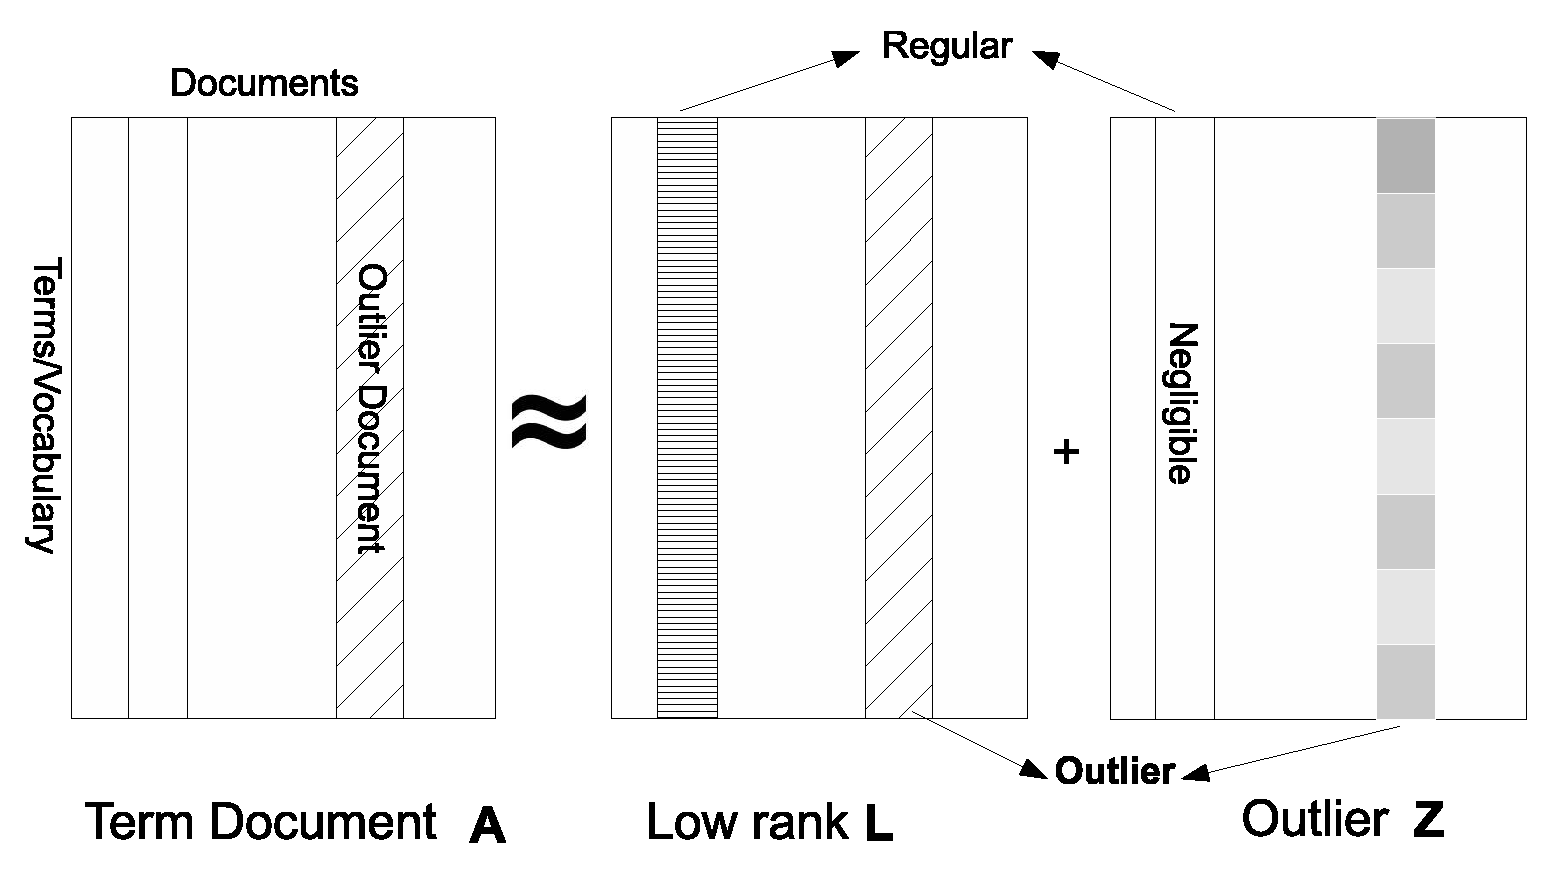
\includegraphics{outlieroverview.eps}}
\caption{Text Outliers Using NMF} \label{fig:outlieroverview}
\end{figure}

Here, $\mathbf{L_0}$ is  a low rank matrix and $\mathbf{Z_0}$
represents the matrix of  outlier entries. Typically, the matrix
$\mathbf{L_0}$ represents the documents created by a lower rank
generative process (such as that modeled by pLSI), and the parts of
the documents that do not correspond to the generative process are
represented as part of the matrix $\mathbf{Z_0}$.   In real world
scenarios, the outlier matrix $\mathbf{Z_0}$  contains  entries
which are very close to zero, and  only a small number of entries
have {\em significantly} non-zero values. These significantly
nonzero entries are often present in only a small fraction of the
columns. Columns which are fully representable in terms of factors
are consistent with the low rank behavior of the data, and therefore
{\em not} outliers. The rank of $\mathbf{L}_0$ is not known in
advance, and it can be expressed in terms of its underlying factors.
$$
\mathbf{L}_0 \approx \mathbf{W}_0\mathbf{H}_0
$$
Here, the two matrices   have dimensions $\mathbf{W}_0 \in
\mathbb{R}^{m \times r}_+$, $\mathbf{H}_0 \in \mathbb{R}^{r \times
n}_+$, and $r \le rank(\mathbf{L}_0)$. The matrices $\mathbf{W}_0$
and  $\mathbf{H}_0$ are non-negative, and this provides
interpretability in terms of being able to express a document as a
non-negative linear combination of the relevant basis vectors, each
of which in itself can be considered a frequency-annotated bag of
words (topics) because of its non-negativity.  Specifically,
$\mathbf{H_0}$ corresponds to the coefficients for the basis matrix
$\mathbf{W_0}$. Intuitively, this corresponds to the case that every
document
 $\mathbf{a}_i$, is represented as the linear combination of
the $r$ topics. In cases, where this is {\em not} true, the document
is an outlier, and those  unrepresentable sections of the matrix are
captured by the non-zero entries in the   $\mathbf{Z_0}$ matrix. In
real scenarios,  the entries in  this matrix are often  extremely
skewed, and the small number of non-zero entries very obviously
expose the outliers.  The decomposition of the matrix into different
component is pictorially illustrated  in Figure
\ref{fig:outlieroverview}.

In order to determine the best low rank factorization, one must try
to optimize the  aggregate  values of the residuals in  the matrix.
This can of course be done in a variety of ways, depending upon the
goals of the underlying factorization process.  We model the
determination of the matrices $\mathbf{W}$,$\mathbf{H}$, and
$\mathbf{Z}$, as the following optimization problem:
\begin{equation}\label{l12norm}
(\mathbf{W}_0,\mathbf{H}_0;\mathbf{Z}_0)=\argmin_{\mathbf{W}\ge0,\mathbf{H}\ge0; \mathbf{Z}}  \frac{1}{2}\norm{\mathbf{A}-\mathbf{W}\mathbf{H}-\mathbf{Z}}_F^2 + \alpha\norm{\mathbf{Z}}_{1,2}
\end{equation}

The specific location of outliers in each column does not have a
closed form solution, since the $\ell_{1,2}$-norm penalty is applied
to $\mathbf{Z}$.   The   logic for applying the $\ell_{1,2}$-norm in
the context of the outlier detection problem is as follows.  Each
entry in the $\mathbf{Z}$ corresponds to a term in a document,
whereas we are interested in the outlier behavior of entire
document. This aggregate outlier behavior of the document $x$ can
be modeled with the $\ell_2$ norm score of a particular column
$\mathbf{z}_x$. In a real scenario,  if a large segment  of a
document $x$ is not representable as the linear combination of the
$r$ topics through $\mathbf{L_0}$, the corresponding column
$\mathbf{z}_x$ in the matrix $\mathbf{Z}$ will be compensated by
having more entries in its column.  In other words, we will  have a
higher $\ell_2$ value for the corresponding column $\mathbf{z}_x$,
and this corresponds to a higher outlier score.
 Furthermore, the  $\ell_{1,2}$-norm penalty on $\mathbf{Z}$
defines the sum of the $\ell_2$ norm outlier scores over all the
documents.  Therefore,  the optimization problem essentially tries
to find the best model,  an important component of which is to
minimize the sum of the outlier scores over all documents.  While a
variety of different  (and more commonly used) penalties such as the
Frobenius norm are available for matrix factorization models, we
have chosen the $\ell_{1,2}$-norm penalty because of its intuitive
significance in the context of the outlier detection problem, and
its tendency to create skewed outlier scores across the columns of
the matrix. As we will see in the next section, this comes at the
expense of a formulation which is more difficult to solve
algorithmically.

For high dimensional data, sparse coefficients are desirable for
obtaining an interpretable low rank matrix $\mathbf{W}\mathbf{H}$.
For this purpose, we add the $\ell_1$-penalty on $\mathbf{H}$:
\begin{equation}\label{outlier}
\min_{\mathbf{W}\ge0,\mathbf{H}\ge0; \mathbf{Z}}  \frac{1}{2}\norm{\mathbf{A}-\mathbf{W}\mathbf{H}-\mathbf{Z}}_F^2 + \alpha\norm{\mathbf{Z}}_{1,2} + \beta\norm{\mathbf{H}}_{1}
\end{equation}
 The constant $\alpha$ defines the weight
for the outlier matrix $\mathbf{Z}$ over the recovery of the low
rank space $\mathbf{L}$ and the sparsity term. In the case of
outlier detection in text documents, we give more weight for the
outlier matrix over the low rank representation $\mathbf{L}$. This
problem does not have a closed form solution, and
 therefore we cannot  directly recover the low rank
matrix $\mathbf{W}\mathbf{H}$ in closed form. However, we can
recover the column space. Without non-negativity constraints, this
property is also known as the rotational invariant property
\cite{ding06,xu12}. This particular formulation of the matrix
factorization model is a bit different from the commonly used
formulations, and off-the-shelf solutions do not directly exist for
this scenario. Therefore, in a later section, we will carefully
design an algorithm with the use of block coordinate descent for
this problem.

In order to understand the modeling of the outliers better, we
present the readers with a toy example from a real world data set,
to show how  skewed the typical values of the corresponding column
$\mathbf{z}(x)$ may be in real scenarios.  In this case, we used the
{\em BBC} dataset\footnote{\url{http://mlg.ucd.ie/datasets/bbc.html}}.
\ramki{This dataset consists of documents from BBC news website corresponding
to stories in area business, entertainment, politics, sport, tech from 2004-2005 . 
%We ran our algorithm \algo explained in the next Section
%\ref{sec:algorithm} to find the matrices $\mathbf{W,H}$ and $\mathbf{Z}$.
We took all the documents from business and politics  and 50
documents from tech labeled as outliers. We randomly permuted the columns to 
shuffle the outliers in the matrix to avoid any spatial bias}. 
We computed the $\mathbf{Z}$ matrix
and   generated the $\ell_2$ scores of the columns of outlier matrix
$\mathbf{Z}$. Figure \ref{fig:outlierz} shows the outlier($\ell_2$)
scores of the documents. The $X$-axis illustrates the index of the
document, and the $Y$-axis illustrates the outlier score. It is
evident that  the scores for some  columns are so close to zero,
that they cannot even be seen on the diagram drawn to scale. These
columns also happened to be the non-outlier/regular documents of the collection.
Such documents $\mathbf{a}_x \in \mathbb{R}^m$ correspond to the low
rank space, and  are approximately representable as  a product of
the basis  matrix $\mathbf{W}$ with the corresponding column vector
of coefficients $\mathbf{h}_x \in \mathbb{R}^r$ drawn from
$\mathbf{H}$. However, the documents that are not representable in
such a low rank space have a large outlier score. From the
distribution of the outlier score, we can also observe that the
scores of outlier documents against non-outliers are clearly
separable, by using a simple statistical mean and standard deviation
analysis. Therefore, while we use the scores to rank the documents
in terms of their outlier behavior, the skew in the entries ensures
that it is often easy to choose a cut-off in order to distinguish
the outliers from the non-outliers.

\begin{figure}
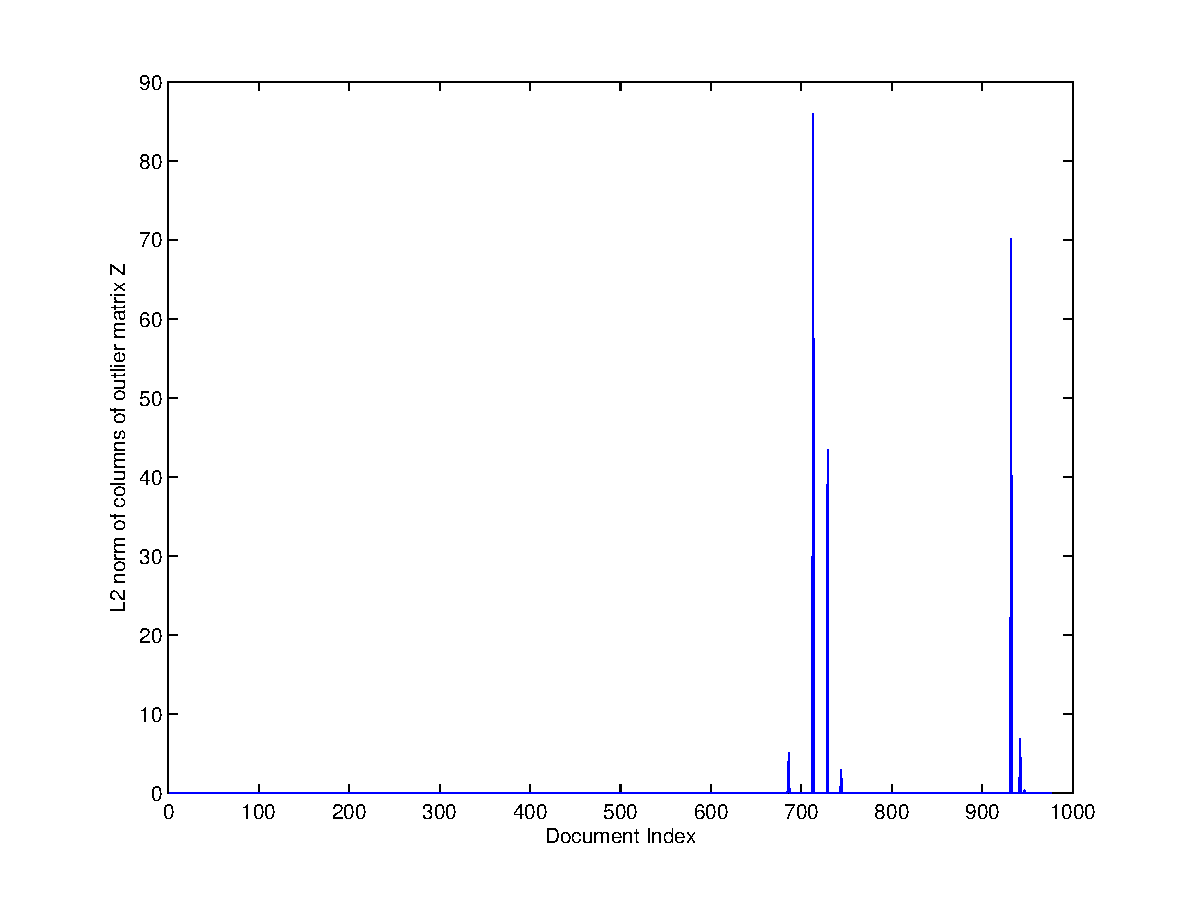
\includegraphics[scale=0.4]{outlierzbbc.eps}
\caption{$\ell_2$ norm of columns of $\mathbf{Z}$ outlier matrix}
\label{fig:outlierz}
\end{figure}



In the following sections, we will analyze the property and
performance of this model \eqref{outlier} for outlier detection
problems.


\section{Algorithm Overview}\label{sec:algorithm}

In analyzing the performance of methods from the previous section, we make two observations:

\begin{enumerate}
\item Global computations (such as a global scan) are expensive, and approaches to multisplit that require many rounds, each with a global computation, are likely to be uncompetitive. Any reduction in the cost of global computation is desirable.
\item After we derive the permutation, the cost of permuting the elements with a global scatter (consecutive input elements going into arbitrarily distant final destinations) is also expensive.
This is primarily because of the non-coalesced memory accesses associated with the scatter. Any increase in memory locality associated with the scatter is also desirable.
\end{enumerate}

The key design insight in this paper is that we can reduce the cost of both global computation and global scatter at the cost of doing more local work, and that doing so is beneficial for overall performance. We begin by describing and analyzing a framework for the different approaches we study in this paper, then discuss the generic structure common to all our implementations.

\subsection{Our parallel model}\label{subsec:parallel_model}
Multisplit cannot be solved by using only local operations; i.e., we cannot divide a multisplit problem into two independent subparts and solve each part locally without any communication between the two parts. We thus assume any viable implementation must include at least a single global operation to gather necessary global information from all elements (or group of elements).
We generalize the approaches we study in this paper into a series of $N$ rounds, where each round has 3 stages: a set of local operations (which run in parallel on independent subparts of the global problem); a global operation (across all subparts); and another set of local operations. In short: \textbraceleft local, global, local\textbraceright, repeated $N$ times; in this paper we refer to these three stages as \textbraceleft prescan, scan, postscan\textbraceright.

The approaches from Section~\ref{sec:init_approaches} all fit this model. Scan-based split starts by making a flag vector (where the local level is per-thread), performing a global scan operation on all flags, and then ordering the results into their final positions (thread-level local). The iterative (or recursive) scan-based split with $m$ buckets repeats the above approach for $m$ (or $\lceil \log m \rceil$) rounds.
Radix sort also requires several rounds. Each round starts by identifying a bit (or a group of bits) from its keys (local), running a global scan operation, and then locally moving data such that all keys are now sorted based on the selected bit (or group of bits).
In radix sort literature, these stages are mostly known as up-sweep, scan and down-sweep.
Reduced-bit sort is derived from radix sort; the main differences are that in the first round, the label vector and the new packed values are generated locally (thread-level), and in the final round, the packed key-value pairs are locally unpacked (thread-level) to form the final results.

\subsection{Multisplit requires a global computation}
Let's explore the global and local components of stable multisplit, which together compute a unique permutation of key-value pairs into their final positions.
Suppose we have $m$ buckets $B_0, B_1, \dots, B_{m-1}$, each with $h_0, h_1, \dots, h_{m-1}$ elements respectively ($\sum_i{h_i} = n$, where $n$ is the total number of elements).
If $u_i \in B_j$ is the $i$th element in key vector $\mathbf{u}$, then its final permuted position $p(i)$ should be (from $u_i$'s perspective):
\begin{equation}\label{eq:permutation}
        p(i) = \underbrace{\sum_{k = 0}^{j-1}h_k}_{\text{global offset}} + \underbrace{\left| \{u_r \in B_j: r < i\}\right|}_{\text{local offset ($u_i$'s bucket)}},
\end{equation}
where $|\cdot|$ is the cardinality operator that denotes the number of elements within its set argument. The left term is the total number of key elements that belong to the preceding buckets, and the right term is the total number of preceding elements (with respect to $u_i$) in $u_i$'s bucket, $B_j$.
Computing both of these terms in this form and for all elements (for all $i$) requires global operations (e.g., computing a histogram of buckets).

\subsection{Dividing multisplit into subproblems}\label{subsec:2levels}
Equation~\eqref{eq:permutation} clearly shows what we need in order to compute each permutation (i.e., final destinations for a stable multisplit solution): a histogram of buckets among all elements ($h_k$) as well as local offsets for all elements within the same bucket (the second term). However, it lacks intuition about how we should compute each term.
Both terms in equation~\eqref{eq:permutation}, at their core, answer the following question: to which bucket does each key belong? If we answer this question for every key and for all buckets (hypothetically, for each bucket we store a binary bitmap variable of length $n$ to show all elements that belong to that bucket), then each term can be computed intuitively as follows: 1)~histograms are equal to counting all elements in each bucket (reduction of a specific bitmap); 2)~local offsets are equivalent to counting all elements from the beginning to that specific index and within the same bucket (scan operation on a specific bitmap).
This intuition is closely related to our definition of the scan-based split method in Section~\ref{sec:scan_split}. However, it is practically not competitive because it requires storing huge bitmaps (total of $mn$ binary variables) and then performing global operations on them.

Although the above solution seems impractical for a large number of keys, it seems more favorable for input problems that are small enough.
As an extreme example, suppose we wish to perform multisplit on a single key. Each bitmap variable becomes just a single binary bit. Performing reduction and scan operations become as trivial as whether a single bit is set or not.
Thus, a divide-and-conquer approach seems like an appealing solution to solve equation~\eqref{eq:permutation}: we would like to divide our main problem into small enough subproblems such that solving each subproblem is ``easy'' for us. By an easy computation we mean that it is either small enough so that we can afford to process it sequentially, or that instead we can use an efficient parallel hardware alternative (such as the GPU's ballot instruction). When we solve a problem directly in this way, we call it a \emph{direct solve}.
Next, we formalize our divide-and-conquer formulation.

Let us divide our input key vector $\mathbf{u}$ into $L$ contiguous subproblems: $\mathbf{u} = [\mathbf{u}_{0}, \mathbf{u}_{1}, \dots, \mathbf{u}_{L-1}]$. Suppose each subvector $\mathbf{u}_\ell$ has $h_{0,\ell}, h_{1,\ell}, \dots, h_{m-1,\ell}$ elements in buckets $B_0, B_1, \dots B_{m-1}$ respectively.
For example, for arbitrary values of $i$, $s$, and $j$ such that key item $u_i \in \mathbf{u}_s$ and $u_i$ is in bucket $B_j$, equation~\eqref{eq:permutation} can be rewritten as (from $u_i$'s perspective):
\begin{equation}\label{eq:permutation2}
p(i) = \underbrace{\overbrace{\sum_{k=0}^{j-1}\left(\sum_{\ell = 0}^{L-1}h_{k,\ell}\right)}^{\text{previous buckets}}+\overbrace{\sum_{\ell=0}^{s-1}h_{j,\ell}}^\text{$u_i$'s bucket}}_\text{global offset}
 + \underbrace{\left| \{u_r \in \mathbf{u}_s: (u_r \in B_j) \land (r < i)\}\right|}_{\text{local offset within $u_i$'s subproblem}}.
 \end{equation}
This formulation has two separate parts. The first and second terms require global computation (first: the element count of all preceding buckets across all subproblems, and second: the element count of the same bucket in all preceding subproblems). The third term can be computed locally within each subproblem. Note that equation~\eqref{eq:permutation} and~\eqref{eq:permutation2}'s first terms are equivalent (total number of previous buckets), but the second term in~\eqref{eq:permutation} is broken into the second and third terms in~\eqref{eq:permutation2}.

The first and second terms can both be computed with a global histogram computed over $L$ local histograms. A global histogram is generally implemented with global scan operations (here, exclusive prefix-sum). We can characterize this histogram as a scan over a 2-dimensional matrix  $\mathbf{H} = [h_{i,\ell}]_{m\times L}$, where the ``height'' of the matrix is the bucket count $m$ and the ``width'' of the matrix is the number of subproblems $L$\@.
The second term can be computed by a scan operation of size $L$ on each row (total of $m$ scans for all buckets). The first term will be a single scan operation of size $m$ over the reduction of all rows (first reduce each row horizontally to compute global histograms and then scan the results vertically). Equivalently, both terms can be computed by a single scan operation of size $mL$ over a row-vectorized $\mathbf{H}$.
Either way, the cost of our global operation is roughly proportional to both $m$ and $L$\@. We see no realistic way to reduce $m$. Thus we concentrate on reducing $L$\@.

\subsection{Hierarchical approach toward multisplit localization}\label{subsec:localization}
We prefer to have small enough subproblems ($\bar{n}$) so that our local computations are ``easy'' for a direct solve. For any given subproblem size, we will have $L = n/\bar{n}$ subproblems to be processed globally as described before.
On the other hand, we want to minimize our global computations as well, because they require synchronization among all subproblems and involve (expensive) global memory accesses.
So, with a fixed input size and a fixed number of buckets ($n$ and $m$), we would like to both decrease our subproblem size and number of subproblems, which is indeed paradoxical.

Our solution is a hierarchical approach. We do an arbitrary number of levels of divide-and-conquer, until at the last level, subproblems are small enough to be solved easily and directly (our preferred $\bar{n}$).
These results are then appropriately combined together to eventually reach the first level of the hierarchy, where now we have a reasonable number of subproblems to be combined together using global computations (our preferred $L$).

Another advantage of such an approach is that, in case our hardware provides a memory hierarchy with smaller but faster local memory storage (as GPUs do with register level and shared memory level hierarchies, as opposed to the global memory), we can potentially perform all computations related to all levels except the first one in our local memory hierarchies without any global memory interaction.
Ideally, we would want to use all our available register and shared memory with our subproblems to solve them locally, and then combine the results using global operations.
In practice, however, since our local memory storage options are very limited, such solution may still lead to a large number of subproblems to be combined with global operations (large $L$).
As a result, by adding more levels of hierarchy (than the available memory hierarchies in our device) we can systematically organize the way we fill our local memories, process them locally, store intermediate results, and then proceed to the next batch, which overall reduces our global operations.
 Next, we will theoretically consider such a hierarchical approach (\emph{multi-level localization}) and explore the changes to equation~\eqref{eq:permutation2}.

\begin{figure}
  \centering
  \begin{tikzpicture}[every node/.style={thick,rectangle,inner sep=0pt}]
\def \dx {0.1}
\def \dy {0.2}
\def \recx {0.15}
\def \recX {5*\recx + 6*\dx}
\def \recXX {3 * \recX + 26 * \dx}
\def \recy {0.75}
\def \recY {\recy + 3 * \dy}
\def \recYY {\recY + 3 * \dy}

%% left child 
\draw [black] (0 + 0, 0 + 0) rectangle (0 + \recx, 0 + \recy);
\draw [black] (0 + \recx + \dx, 0) rectangle (0 + 2*\recx + \dx, 0 + \recy);
\draw [black] (0 + 2*\recx + 2*\dx, 0 + 0) rectangle (0 + 3*\recx + 2*\dx, 0 + \recy);
\draw [black] (0 + 3*\recx + 3*\dx, 0 + 0) rectangle (0 + 4*\recx + 3*\dx, 0 + \recy);
\draw [black] (0 + 4*\recx + 4*\dx, 0 + 0) rectangle (0 + 5*\recx + 4*\dx, 0 + \recy);

\draw[thick, black] (0-2*\dx, 0-\dy) rectangle (0-2*\dx + \recX + 2 * \dx, 0-\dy + \recY);
\node () at (0 + 2 * \recx + 3 * \dx, \recy + \dy) {$L_2$};

\draw [black] (\recX + 4*\dx + 0, 0 + 0) rectangle (\recX + 4*\dx + \recx, 0 + \recy);
\draw [black] (\recX + 4*\dx + \recx + \dx, 0) rectangle (\recX + 4*\dx + 2*\recx + \dx, 0 + \recy);
\draw [black] (\recX + 4*\dx + 2*\recx + 2*\dx, 0 + 0) rectangle (\recX + 4*\dx + 3*\recx + 2*\dx, 0 + \recy);
\draw [black] (\recX + 4*\dx + 3*\recx + 3*\dx, 0 + 0) rectangle (\recX + 4*\dx + 4*\recx + 3*\dx, 0 + \recy);
\draw [black] (\recX + 4*\dx + 4*\recx + 4*\dx, 0 + 0) rectangle (\recX + 4*\dx + 5*\recx + 4*\dx, 0 + \recy);

\draw[thick, black] (\recX + 4*\dx-2*\dx, 0-\dy) rectangle (\recX + 4*\dx-2*\dx + \recX + 2 * \dx, 0-\dy + \recY);
\node () at (\recX + 4*\dx + 2 * \recx + 3 * \dx, \recy + \dy) {$L_2$};

\draw [black] (2*\recX + 14*\dx + 0, 0 + 0) rectangle (2*\recX + 14*\dx + \recx, 0 + \recy);
\draw [black] (2*\recX + 14*\dx + \recx + \dx, 0) rectangle (2*\recX + 14*\dx + 2*\recx + \dx, 0 + \recy);
\draw [black] (2*\recX + 14*\dx + 2*\recx + 2*\dx, 0 + 0) rectangle (2*\recX + 14*\dx + 3*\recx + 2*\dx, 0 + \recy);
\draw [black] (2*\recX + 14*\dx + 3*\recx + 3*\dx, 0 + 0) rectangle (2*\recX + 14*\dx + 4*\recx + 3*\dx, 0 + \recy);
\draw [black] (2*\recX + 14*\dx + 4*\recx + 4*\dx, 0 + 0) rectangle (2*\recX + 14*\dx + 5*\recx + 4*\dx, 0 + \recy);

\draw[thick, black] (2*\recX + 14*\dx-2*\dx, 0-\dy) rectangle (2*\recX + 14*\dx-2*\dx + \recX + 2 * \dx, 0-\dy + \recY);
\node () at (2*\recX + 14*\dx + 2 * \recx + 3 * \dx, \recy + \dy) {$L_2$};

\draw [thick, black] (0-4*\dx, 0-2*\dy) rectangle (0-4*\dx + \recXX, 0-2*\dy + \recYY);
\node () at (\recX + 4*\dx + 2 * \recx + 3 * \dx, \recy + 3* \dy) {$L_1$};

%% second tile
\draw [black] (\recXX + 4*\dx + 0, 0 + 0) rectangle (\recXX + 4 * \dx + \recx, 0 + \recy);
\draw [black] (\recXX + 4*\dx + \recx + \dx, 0) rectangle (\recXX + 4 * \dx + 2*\recx + \dx, 0 + \recy);
\draw [black] (\recXX + 4*\dx + 2*\recx + 2*\dx, 0 + 0) rectangle (\recXX + 4 * \dx + 3*\recx + 2*\dx, 0 + \recy);
\draw [black] (\recXX + 4*\dx + 3*\recx + 3*\dx, 0 + 0) rectangle (\recXX + 4 * \dx + 4*\recx + 3*\dx, 0 + \recy);
\draw [black] (\recXX + 4*\dx + 4*\recx + 4*\dx, 0 + 0) rectangle (\recXX + 4 * \dx + 5*\recx + 4*\dx, 0 + \recy);

\draw[thick, black] (\recXX + 4*\dx-2*\dx, 0-\dy) rectangle (\recXX + 4 * \dx-2*\dx + \recX + 2 * \dx, 0-\dy + \recY);
\node () at (\recXX + 4*\dx + 3*\dx + 2 * \recx, \recy + \dy) {$L_2$};

\draw [black] (\recXX + 4*\dx + \recX + 4*\dx + 0, 0 + 0) rectangle (\recXX + 4*\dx + \recX + 4*\dx + \recx, 0 + \recy);
\draw [black] (\recXX + 4*\dx + \recX + 4*\dx + \recx + \dx, 0) rectangle (\recXX + 4*\dx + \recX + 4*\dx + 2*\recx + \dx, 0 + \recy);
\draw [black] (\recXX + 4*\dx + \recX + 4*\dx + 2*\recx + 2*\dx, 0 + 0) rectangle (\recXX + 4*\dx + \recX + 4*\dx + 3*\recx + 2*\dx, 0 + \recy);
\fill [green] (\recXX + 4*\dx + \recX + 4*\dx + 3*\recx + 3*\dx, 0 + 0) rectangle (\recXX + 4*\dx + \recX + 4*\dx + 4*\recx + 3*\dx, 0 + \recy);
\draw [black] (\recXX + 4*\dx + \recX + 4*\dx + 3*\recx + 3*\dx, 0 + 0) rectangle (\recXX + 4*\dx + \recX + 4*\dx + 4*\recx + 3*\dx, 0 + \recy);
\draw [black] (\recXX + 4*\dx + \recX + 4*\dx + 4*\recx + 4*\dx, 0 + 0) rectangle (\recXX + 4*\dx + \recX + 4*\dx + 5*\recx + 4*\dx, 0 + \recy);

\draw[thick, black] (\recXX + 4*\dx + \recX + 4*\dx-2*\dx, 0-\dy) rectangle (\recXX + 4*\dx + \recX + 4*\dx-2*\dx + \recX + 2 * \dx, 0-\dy + \recY);
\node () at (\recXX + 4*\dx + \recX + 4*\dx + 2 * \recx + 3 * \dx, \recy + \dy) {$L_2$};

\draw [black] (\recXX + 4*\dx + 2*\recX + 14*\dx + 0, 0 + 0) rectangle (\recXX + 4*\dx + 2*\recX + 14*\dx + \recx, 0 + \recy);
\draw [black] (\recXX + 4*\dx + 2*\recX + 14*\dx + \recx + \dx, 0) rectangle (\recXX + 4*\dx + 2*\recX + 14*\dx + 2*\recx + \dx, 0 + \recy);
\draw [black] (\recXX + 4*\dx + 2*\recX + 14*\dx + 2*\recx + 2*\dx, 0 + 0) rectangle (\recXX + 4*\dx + 2*\recX + 14*\dx + 3*\recx + 2*\dx, 0 + \recy);
\draw [black] (\recXX + 4*\dx + 2*\recX + 14*\dx + 3*\recx + 3*\dx, 0 + 0) rectangle (\recXX + 4*\dx + 2*\recX + 14*\dx + 4*\recx + 3*\dx, 0 + \recy);
\draw [black] (\recXX + 4*\dx + 2*\recX + 14*\dx + 4*\recx + 4*\dx, 0 + 0) rectangle (\recXX + 4*\dx + 2*\recX + 14*\dx + 5*\recx + 4*\dx, 0 + \recy);

\draw[thick, black] (\recXX + 4*\dx + 2*\recX + 14*\dx-2*\dx, 0-\dy) rectangle (\recXX + 4*\dx + 2*\recX + 14*\dx-2*\dx + \recX + 2 * \dx, 0-\dy + \recY);
\node () at (\recXX + 4*\dx + 2*\recX + 14*\dx + 2 * \recx + 3 * \dx, \recy + \dy) {$L_2$};

\draw [thick, black] (\recXX + 4*\dx + 0-4*\dx, 0-2*\dy) rectangle (\recXX + 4*\dx + 0-4*\dx + \recXX, 0-2*\dy + \recYY);
\node () at (\recXX + 4*\dx + \recX + 4*\dx + 2 * \recx + 3 * \dx, \recy + 3* \dy) {$L_1$};

%% outer rectangle:
\draw [thick, black] (0-6*\dx, 0 - 3 * \dy) rectangle (0-6*\dx + 3*\recXX + 12*\dx + 6*\dx, 0-3*\dy + \recYY + 3*\dy);
\node () at (\recXX -2* \dx, \recYY -\dy) {$L_0$};

% \def\dx{1}
% \def\a{0}
% \def\recx{0.15}
% \def\recy{0.75}
% \node (a1) at (0 * \dx,0) [draw, minimum width=\recx cm, minimum height=\recy cm, anchor=north] {};
% \node (ap1) at (0.25 * \dx,0) [draw, minimum width=\recx cm, minimum height=\recy cm, anchor=north] {};
% \node (ap1) at (0.5 * \dx,0) [draw, minimum width=\recx cm, minimum height=\recy cm, anchor=north] {};
% \node (ap1) at (0.75 * \dx,0) [draw, minimum width=\recx cm, minimum height=\recy cm, anchor=north] {};
% \node (a2) at (1*\dx,0) [draw, minimum width=\recx cm, minimum height=\recy cm, anchor=north] {};

% \node (a3) at (2*\dx,0) [draw, minimum width=\recx cm, minimum height=\recy cm, anchor=north] {};
% \node (ap3) at (2.25*\dx,0) [draw, minimum width=\recx cm, minimum height=\recy cm, anchor=north] {};
% \node (ap3) at (2.5*\dx,0) [draw, minimum width=\recx cm, minimum height=\recy cm, anchor=north] {};
% \node (ap3) at (2.75*\dx,0) [draw, minimum width=\recx cm, minimum height=\recy cm, anchor=north] {};
% \node (a4) at (3*\dx,0) [draw, minimum width=\recx cm, minimum height=\recy cm, anchor=north] {};

% \node (a5) at (4*\dx,0) [draw, minimum width=\recx cm, minimum height=\recy cm, anchor=north] {};
% \node (ap5) at (4.25*\dx,0) [draw, minimum width=\recx cm, minimum height=\recy cm, anchor=north] {};
% \node (ap5) at (4.5*\dx,0) [draw, minimum width=\recx cm, minimum height=\recy cm, anchor=north] {};
% \node (ap5) at (4.75*\dx,0) [draw, minimum width=\recx cm, minimum height=\recy cm, anchor=north] {};
% \node (a6) at (5*\dx,0) [draw, minimum width=\recx cm, minimum height=\recy cm, anchor=north] {};

% \node (a7) at (6*\dx + \a,0) [draw, minimum width=\recx cm, minimum height=\recy cm, anchor=north] {};
% \node (ap7) at (6.25*\dx + \a,0) [draw, minimum width=\recx cm, minimum height=\recy cm, anchor=north] {};
% \node (ap7) at (6.5*\dx + \a,0) [draw, minimum width=\recx cm, minimum height=\recy cm, anchor=north] {};
% \node (ap7) at (6.75*\dx + \a,0) [draw, minimum width=\recx cm, minimum height=\recy cm, anchor=north] {};
% \node (a8) at (7*\dx+ \a,0) [draw, minimum width=\recx cm, minimum height=\recy cm, anchor=north] {};

% \node (a9) at (8*\dx+ \a,0) [draw, minimum width=\recx cm, minimum height=\recy cm, anchor=north] {};
% \node (ap9) at (8.25*\dx+ \a,0) [draw, minimum width=\recx cm, minimum height=\recy cm, anchor=north] {};
% \node (ap9) at (8.5*\dx+ \a,0) [draw, minimum width=\recx cm, minimum height=\recy cm, anchor=north] {};
% \node (app9) at (8.75*\dx+ \a,0) [draw, minimum width=\recx cm, minimum height=\recy cm, anchor=north, fill=green] {};
% \node (a10) at (9*\dx+ \a,0) [draw, minimum width=\recx cm, minimum height=\recy cm, anchor=north] {};

% \draw[->] (app9) -- (8.75*\dx + \a, -1.65);
% \node (text) at (8.75*\dx + \a + 0.1, -1.75) {\scriptsize$(1,1,3)$};

% \node (a11) at (10*\dx+ \a,0) [draw, minimum width=\recx cm, minimum height=\recy cm, anchor=north] {};
% \node (ap11) at (10.25*\dx+ \a,0) [draw, minimum width=\recx cm, minimum height=\recy cm, anchor=north] {};
% \node (ap11) at (10.5*\dx+ \a,0) [draw, minimum width=\recx cm, minimum height=\recy cm, anchor=north] {};
% \node (ap11) at (10.75*\dx+ \a,0) [draw, minimum width=\recx cm, minimum height=\recy cm, anchor=north] {};
% \node (a12) at (11*\dx+ \a,0) [draw, minimum width=\recx cm, minimum height=\recy cm, anchor=north] {};

% \node (b1) [draw, minimum width=10*\recx cm, minimum height=2*\recy cm, anchor=north, label=$L_2$, fit = (a1)(a2), rounded corners=0.1cm] {};
% \node (b2) [draw, minimum width=10*\recx cm, minimum height=2*\recy cm, anchor=north, label=$L_2$, fit = (a3)(a4), rounded corners=0.1cm] {};
% \node (b3) [draw, minimum width=10*\recx cm, minimum height=2*\recy cm, anchor=north, label=$L_2$, fit = (a5)(a6), rounded corners=0.1cm] {};

% \node (b4) [draw, minimum width=10*\recx cm, minimum height=2*\recy cm, anchor=north, label=$L_2$, fit = (a7)(a8), rounded corners=0.1cm] {};
% \node (b5) [draw, minimum width=10*\recx cm, minimum height=2*\recy cm, anchor=north, label=$L_2$, fit = (a9)(a10), rounded corners=0.1cm] {};
% \node (b6) [draw, minimum width=10*\recx cm, minimum height=2*\recy cm, anchor=north, label=$L_2$, fit = (a11)(a12), rounded corners=0.1cm] {};

% \node (c1) [draw, minimum width=38*\recx cm, minimum height=3* \recy cm, anchor=north, label=$L_1$, fit = (b1)(b2)(b3), rounded corners=0.1cm] {};
% \node (c2) [draw, minimum width=38*\recx cm, minimum height=3* \recy cm, anchor=north, label=$L_1$, fit = (b4)(b5)(b6), rounded corners=0.1cm] {};

% \node (d1) [draw, minimum width=80*\recx cm, minimum height=4 * \recy cm, anchor=north, label=$L_0$, fit = (c1)(c2), rounded corners=0.1cm] {};

\end{tikzpicture}
  \caption{An example for our localization terminology. Here we have 3 levels of localization with $L_0 = 2$, $L_1 = 3$ and $L_2 = 5$. For example, the marked subproblem (in green) can be addressed by a tuple $(1,1,3)$ where each index respectively denotes its position in the hierarchical structure.\label{fig:localization}}
\end{figure}

% Consider a hierarchical approach, such that we continue our divisions: we divide each subproblem into several smaller subsubproblems, and continue to do so.
\paragraph{$\lambda$-level localization}
For any given set of arbitrary non-zero integers $\{L_0, L_1, \dots, L_{\lambda - 1}\}$, we can perform $\lambda$ levels of localizations as follows: Suppose we initially divide our problem into $L_0$ smaller parts. These divisions form our first level (i.e., the \emph{global level}).
Next, each subproblem at the first level is divided into $L_1$ smaller subproblems to form the second level. We continue this process until the $\lambda$th level (with $L_{\lambda-1}$ subproblems each). Figure~\ref{fig:localization} shows an example of our hierarchical division of the multisplit problem.
There are total of $L_\text{total} = L_0 \times L_1 \times \dots L_{\lambda - 1}$ smaller problems and their results should be hierarchically added together to compute the final permutation $p(i)$.
Let $(\ell_0,\ell_1,\dots,\ell_{\lambda-1})$ denote a subproblem's position in our hierarchical tree: $\ell_0$th branch from the first level, $\ell_1$th branch from the second level, and so forth until the last level.
Among all elements within this subproblem, we count those that belong to bucket $B_i$ as $h_{i,(\ell_0,\dots,\ell_{\lambda-1})}$.
Similar to our previous permutation computation, for an arbitrary $i$, $j$, and $(s_0,\dots,s_{\lambda-1})$, suppose $u_i \in \mathbf{u}_{(s_0, \dots, s_{\lambda-1})}$ and $u_i \in B_j$.
We can write $p(i)$ as follows (from $u_i$'s perspective):

\begin{IEEEeqnarray}{rCl}\label{eq:permutation3}
p(i) & = & \sum_{k = 0}^{j-1}\left(\sum_{\ell_0 = 0}^{L_0 - 1} \sum_{\ell_1 = 0}^{L_1 - 1} \dots \sum_{\ell_{\lambda - 1} = 0}^{L_{\lambda - 1} - 1}h_{k, (\ell_0, \ell_1, \dots, \ell_{\lambda-1})}\right)
\hfill \rightarrow \text{\scriptsize previous buckets in the whole problem} \nonumber \\
&& +\: \sum_{\ell_0 = 0}^{s_0 - 1}\left(\sum_{\ell_1 = 0}^{L_1-1}\dots\sum_{\ell_{\lambda-1}=0}^{L_{\lambda-1} - 1}{h_{j,(\ell_0,\ell_1,\dots,\ell_{\lambda-1})}}\right)
\hfill\rightarrow \text{\scriptsize $u_i$'s bucket, first level, previous subproblems} \nonumber \\
&& +\: \sum_{\ell_1 = 0}^{s_1 - 1}\left(\sum_{\ell_2 = 0}^{L_2-1}\dots\sum_{\ell_{\lambda-1}=0}^{L_{\lambda-1} - 1}{h_{j,(s_0,\ell_1,\ell_2,\dots,\ell_{\lambda-1})}}\right)
\hfill\rightarrow \text{\scriptsize $u_i$'s bucket, second level, previous subproblems} \nonumber \\
&& \vdots \hfill\rightarrow \text{\scriptsize $u_i$'s bucket, previous levels, previous subproblems} \nonumber \\
&& +\: \sum_{\ell_{\lambda-1} = 0}^{s_{\lambda-1} - 1}h_{j,(s_0,\dots,s_{\lambda-2},\ell_{\lambda-1})}
\hfill\rightarrow \text{\scriptsize $u_i$'s bucket, last level, previous subproblems} \nonumber \\
&& +\: \left| \left\{u_r \in \mathbf{u}_{(s_0, \dots, s_{\lambda-1})}: (u_r \in B_j) \land (r < i)\right\}\right|.
\hfill\rightarrow \text{\scriptsize $u_i$'s bucket, $u_i$'s subproblem} \nonumber \\
\end{IEEEeqnarray}

There is an important resemblance between this equation and equation~\eqref{eq:permutation2}. The first and second terms (from top to bottom) are similar, with the only difference that each $h_{k,\ell}$ is now further broken into $L_1\times \dots \times L_{\lambda-1}$ subproblems (previously it was just $L = L_0$ subproblems). The other terms of \eqref{eq:permutation3} can be seen as a hierarchical disintegration of the local offset in \eqref{eq:permutation2}.

Similar to Section~\ref{subsec:2levels}, we can form a matrix $\mathbf{H} = [h_{j,\ell_0}]_{m\times L_0}$ for global computations where
\begin{equation}
h_{j,\ell_0} = \sum_{\ell_1 = 0}^{L_1-1}\dots\sum_{\ell_{\lambda-1} = 0}^{L_{\lambda-1}-1} h_{j, (\ell_0, \ell_1,\dots,\ell_{\lambda-1})}.
\end{equation}
Figure~\ref{fig:localization_matrix} depicts an schematic example of multiple levels of localization.
At the highest level, for any arbitrary subproblem $(\ell_0,\ell_1\dots,\ell_{\lambda-1})$, local offsets per key are computed as well as all bucket counts. Bucket counts are then summed and sent to a lower level to form the bucket count for more subproblems ($L_{\lambda-1}$ consecutive subproblems). This process is continued until reaching the first level (the global level) where we have bucket counts for each $L_1\times\dots\times L_{\lambda-1}$ consecutive subproblems. This is where $\mathbf{H}$ is completed, and we can proceed with our global computation. Next, we discuss the way we compute local offsets.

\begin{figure}
  \centering
  \begin{tikzpicture}[every node/.style={thick,rectangle,inner sep=0pt}]
\def\recB{3.5}
\def\recX{3.5}
\def\recXX{3.5}
\def\recXXX{3.5}
\def\aXX{0.5}
\def\recY{0.5}
\def\midX{0.75}
\def \a {0.6}
\node (d1) at (0 * \recB, 1.5) [draw=black,rectangle,minimum width = \recB cm, minimum height = \recY cm] {\small$0$th row of $\mathbf{H}$};
\node (md1) [right=-1pt of d1, draw=black,rectangle,minimum width = \midX cm, minimum height = \recY cm] {$\dots$};
\node (d2) [right=-1pt of md1,draw=black,rectangle,minimum width = \recB cm, minimum height = \recY cm] {\small$j$th row of $\mathbf{H}$};
\node (md2) [right=-1pt of d2, draw=black,rectangle,minimum width = \midX cm, minimum height = \recY cm] {$\dots$};
\node (d3) [right=-1pt of md2,draw=black,rectangle,minimum width = \recB cm, minimum height = \recY cm] {\small($m-1$)th row of $\mathbf{H}$};
\node at (d1.north) [anchor=south] {$B_0$};
\node at (d2.north) [anchor=south] {$B_j$};
\node at (d3.north) [anchor=south] {$B_{m-1}$};

\node (a1) at (0 * \recX + \aXX, 0) [draw=black,rectangle,minimum width = \recX cm, minimum height = \recY cm] {$h_{j, (0, \ast, \dots, \ast)}$};
\node (m1) [right=-1pt of a1, draw=black,rectangle,minimum width = \midX cm, minimum height = \recY cm] {$\dots$};
\node (a2) [right=-1pt of m1,draw=black,rectangle,minimum width = \recX cm, minimum height = \recY cm] {$h_{j, (\ell_0, \ast, \dots, \ast)}$};
\node (m2) [right=-1pt of a2, draw=black,rectangle,minimum width = \midX cm, minimum height = \recY cm] {$\dots$};
\node (a3) [right=-1pt of m2,draw=black,rectangle,minimum width = \recX cm, minimum height = \recY cm] {$h_{j, (L_{0} - 1, \ast, \dots, \ast)}$};

\node (sum1) [below=8pt of a2] {\large$\sum$};
\node at (a1.north) [anchor=south] {$H_{j,0}$};
\node at (a2.north) [anchor=south] {$H_{j,\ell_0}$};
\node at (a3.north) [anchor=south] {$H_{j, L_0-1}$};


\node (b1) at (0 * \recXX + 2*\aXX, -1.5) [draw=black,rectangle,minimum width = \recXX cm, minimum height = \recY cm] {$h_{j, (\ell_0, 0, \ast, \dots, \ast)}$};
\node (mb1) [right=-1pt of b1, draw=black,rectangle,minimum width = \midX cm, minimum height = \recY cm] {$\dots$};
\node (b2) [right=-1pt of mb1,draw=black,rectangle,minimum width = \recXX cm, minimum height = \recY cm] {$h_{j, (\ell_0, \ell_1, \ast, \dots, \ast)}$};
\node (mb2) [right=-1pt of b2, draw=black,rectangle,minimum width = \midX cm, minimum height = \recY cm] {$\dots$};
\node (b3) [right=-1pt of mb2,draw=black,rectangle,minimum width = \recXX cm, minimum height = \recY cm] {$h_{j, (\ell_0, L_{1} - 1, \ast, \dots, \ast)}$};

\node (sum2) [below=8pt of b2] {\large$\sum$};

\draw [thick, black, dashed] (a2.south west) -- (b1.north west);
\draw [thick, black, dashed] (a2.south east) -- (b3.north east);

\node (c1) at (0 * \recXXX + 3*\aXX, -3) [draw=black,rectangle,minimum width = \recXXX cm, minimum height = \recY cm] {$h_{j, (\ell_0, \ell_1, 0,  \ast, \dots, \ast)}$};
\node (mc1) [right=-1pt of c1, draw=black,rectangle,minimum width = \midX cm, minimum height = \recY cm] {$\dots$};
\node (c2) [right=-1pt of mc1,draw=black,rectangle,minimum width = \recXXX cm, minimum height = \recY cm] {$h_{j, (\ell_0, \ell_1, \ell_2,\ast,  \dots, \ast)}$};
\node (mc2) [right=-1pt of c2, draw=black,rectangle,minimum width = \midX cm, minimum height = \recY cm] {$\dots$};
\node (c3) [right=-1pt of mc2,draw=black,rectangle,minimum width = \recXXX cm, minimum height = \recY cm] {$h_{j, (\ell_0, \ell_1, L_{2} - 1, \ast, \dots, \ast)}$};

\draw [thick, black, dashed] (b2.south west) -- (c1.north west);
\draw [thick, black, dashed] (b2.south east) -- (c3.north east);

\draw [thick, black, dashed] (d2.south west) -- (a1.north west);
\draw [thick, black, dashed] (d2.south east) -- (a3.north east);

\node (dots1) [below=4pt of c2] {\large$\ddots$};

\node (e1) at (0 * \recXXX + 3.5*\aXX, -4.5) [draw=black,rectangle,minimum width = \recXXX cm, minimum height = \recY cm] {$h_{j, (\ell_0, \ell_1, \dots, 0)}$};
\node (me1) [right=-1pt of e1, draw=black,rectangle,minimum width = \midX cm, minimum height = \recY cm] {$\dots$};
\node (e2) [right=-1pt of me1,draw=black,rectangle,minimum width = \recXXX cm, minimum height = \recY cm] {$h_{j, (\ell_0, \ell_1, \dots, \ell_{\lambda-1})}$};
\node (me2) [right=-1pt of e2, draw=black,rectangle,minimum width = \midX cm, minimum height = \recY cm] {$\dots$};
\node (e3) [right=-1pt of me2,draw=black,rectangle,minimum width = \recXXX cm, minimum height = \recY cm] {$h_{j, (\ell_0, \ell_1, \dots, L_{\lambda-1})}$};

\node (sum3) [below=12pt of e2,draw,circle, inner sep=3pt]{\large $6$};

\def\inputKeys{{"*","B_j","*","*","B_j","B_j","*","*","B_j","*","*","B_j","*","*","B_j","*"}}

\def\localOffset{{"*","0","*","*","1","2","*","*","3","*","*","4","*","*","5","*"}}

\node (A) at (0 * \recXXX + 4*\aXX, -6.5) [minimum height = \recY cm] {\text{buckets    }};
\node (l) [below=0pt of A, minimum height = \recY cm] {\small\text{local offset  }};
\foreach \x in {0,...,15}{
	\node (A) [right=-1pt of A, draw=black,rectangle,minimum width = \a cm, minimum height = \recY cm] {$\pgfmathparse{\inputKeys[\x]}\pgfmathresult$};
	\node (l) [below=6pt of A] {$\pgfmathparse{\localOffset[\x]}\pgfmathresult$};
	\ifthenelse{\x=1 \OR \x=4 \OR \x=5 \OR \x=8 \OR \x=11 \OR \x=14}{\draw(A.north)--(sum3);}{}	
}

\draw [thick,black] (sum3.north) -- (e2.south);
\end{tikzpicture}
  \caption{Each row of $\mathbf{H}$ belongs to a different bucket. Results from different subproblems in different levels are added together to form a lower level bucket count. This process is continued until reaching the first level where $\mathbf{H}$ is completed.\label{fig:localization_matrix}}
\end{figure}

\subsection{Direct solve: Local offset computation}
At the very last level of our localization,
each element must compute its own local offset, which represents the number of elements in its subproblem (with our preferred size $\bar{n}$) that both precede it and share its bucket.
To compute local offsets of a subproblem of size $\bar{n}$, we  make a new binary matrix $\bar{\mathbf{H}}_{m\times \bar{n}}$, where each row represents a bucket and each column represents a key element.
Each entry of this new matrix is one if the corresponding key element belongs to that bucket, and zero otherwise.
Then by performing an exclusive scan on each row, we can compute local offsets for all elements belonging to that row (bucket). So each subproblem requires the following computations:
\begin{enumerate}
        \item Mark all elements in each bucket (making local $\bar{\mathbf{H}}$)
        \item $m$ local reductions over the rows of $\bar{\mathbf{H}}$ to compute local histograms (a column in $\mathbf{H}$)
        \item $m$ local exclusive scans on rows of $\bar{\mathbf{H}}$ (local offsets)
\end{enumerate}
For clarity, we separate steps 2 and 3 above, but we can achieve both with a single local scan operation.
Step 2 provides all histogram results that we need in equations~\eqref{eq:permutation2} or \eqref{eq:permutation3} (i.e., all $h_{k, (\ell_0, \dots, \ell_{\lambda-1})}$ values) and step 3 provides the last term in either equation (Fig.~\ref{fig:localization_matrix}).

It is interesting to note that as an extreme case of localization, we can have $L = n$ subproblems, where we divide our problem so much that in the end each subproblem is a single element. In such case, $\bar{\mathbf{H}}$ is itself a binary value. Thus, step 2's result is either 0 or 1. The local offset (step 3) for such a singleton matrix is always a zero (there is no other element within that subproblem).

\subsection{Our multisplit algorithm}

Now that we've outlined the different computations required for the multisplit, we can present a high-level view of the algorithmic skeleton we use in this paper. We require three steps:

\begin{enumerate}
\item \emph{Local}. For each subproblem at the highest level of our localization, for each bucket, count the number of items in the subproblem that fall into that bucket (direct solve for bucket counts).
Results are then combined hierarchically and locally (based on equation~\eqref{eq:permutation3}) until we have bucket counts per subproblem for the first level (global level).
\item \emph{Global}. Scan the bucket counts for each bucket across all subproblems in the first level (global level), then scan the bucket totals. Each subproblem now knows both a)~for each bucket, the total count for all its previous buckets across the whole input vector (term 1 in equation~\eqref{eq:permutation3}) and b)~for each bucket, the total count from the previous subproblems  (term 2 in equation~\eqref{eq:permutation3}).
\item \emph{Local}. For each subproblem at the highest level of our localization, for each item, recompute bucket counts and compute the local offset for that item's bucket (direct solve).
Local results for each level are then appropriately combined together with the global results from the previous levels (based on equation~\eqref{eq:permutation3}) to compute final destinations.
We can now write each item in parallel into its location in the output vector.
\end{enumerate}

\subsection{Reordering elements for better locality}\label{subsec:alg_reordering}
After computing equation~\eqref{eq:permutation3} for each key element, we can move key-value pairs to their final positions in global memory. However, in general, any two consecutive key elements in the original input do not belong to the same bucket, and thus their final destination might be far away from each other (i.e., a global scatter).
Thus, when we write them back to memory, our memory writes are poorly coalesced, and our achieved memory bandwidth during this global scatter is similarly poor. This results in a huge performance bottleneck. How can we increase our coalescing and thus the memory bandwidth of our final global scatter?
Our solution is to \emph{reorder} our elements within a subproblem at the lowest level (or any other higher level) before they are scattered back to memory.
Within a subproblem, we attempt to place elements from the same bucket next to each other, while still preserving order within a bucket (and thus the stable property of our multisplit implementation). We do this reordering at the same time we compute local offsets in equation~\eqref{eq:permutation2}. How do we group elements from the same bucket together? A local multisplit within the subproblem!

We have already computed histogram and local offsets for each element in each subproblem. We only need to perform another local exclusive scan on local histogram results to compute new positions for each element in its subproblem (computing equation~\eqref{eq:permutation} for each subproblem).
We emphasize that performing this additional stable multisplit on each subproblem does \emph{not} change its histogram and local offsets, and hence does not affect any of our computations described previously from a global perspective; the final multisplit result is identical. But, it has a significant positive impact on the locality of our final data writes to global memory.

It is theoretically better for us to perform reordering in our largest subproblems (first level) so that there are potentially more candidate elements that might have consecutive/nearby final destinations.
However, in practice, we may prefer to reorder elements in higher levels, not because they provide better locality but for purely practical limitations (such as limited available local memory to contain all elements within that subproblem).

% \subsection{Choosing the size of subproblems}
% The traditional approach to both histograms and multisplit (as in He et al.~\cite{He:2008:RJG}) is to assign the $n$ elements to $n$ threads\footnote{We might apply thread coarsening---multiple items per thread---and divide $n$ by the number of items per thread.} and treat them as $n$ separate subproblems. This approach is simple: with it, ``local'' work is minimal, even trivial, and the scan implementation at the core of the global operation will typically transparently leverage the GPU's computation hierarchy. Nonetheless, a scan of size $n$ is still more expensive than we would like.

% GPUs offer many potential natural subproblem sizes that correspond to the levels of their computational hierarchies: problems the size of threads, warps, blocks, and the entire device (global). We have shown above that choosing larger subproblems is possible, and in the next section how we can implement their operations efficiently. We thus face a performance tradeoff. With a large $L$, local computations are easier because each subproblem has fewer elements, but global operations will cost more because $\mathbf{H}$ is larger. On the other hand, a smaller $L$ (fewer subproblems) leads to cheaper global operations, but also larger subproblems and hence more expensive local computation.


\section{Experimental Evaluation}
\label{sec:exp}
We are using using three different settings, $Setting = [\lambda_1, \lambda_2, \lambda_3]$, in the experiments. In $Setting_1 = [1.6, 0.35, 0.05]$, the average interaction involved three nodes (a triad), which corresponds approximately to the analyzed co-authorship network. This setting presumes the interaction is dominated by neighbors of the proactive node with the occasional participation of new nodes and rather exceptional participation of existing nodes yet not connected to the proactive node. In $Setting_2 = [3, 6, 1]$ predominate new nodes, and the average number of nodes in interaction is $11$. In $Setting_3 = [0.45, 0.45, 0.1]$ interaction involved two nodes (a dyad) on average, wherein the number of neighbors and new nodes are balanced and new connection occurrences are less likely.

\begin{figure}[ht]
	\centering
  \begin{subfigure}{2.7cm}
    \centering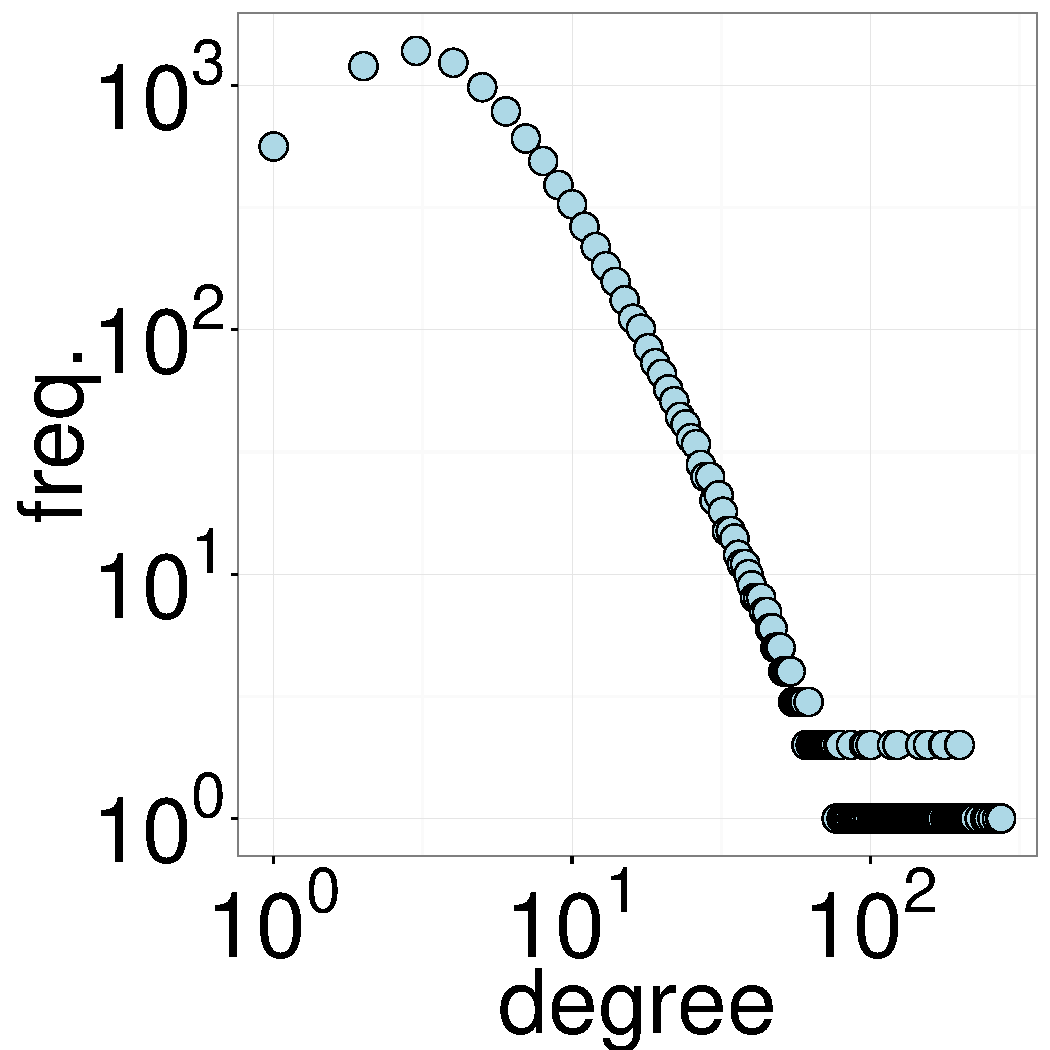
\includegraphics[width=2.5cm]{figures/distr_stupnu_Setting1}
    \caption{$Setting_1$}
  \end{subfigure}
  \begin{subfigure}{2.7cm}
    \centering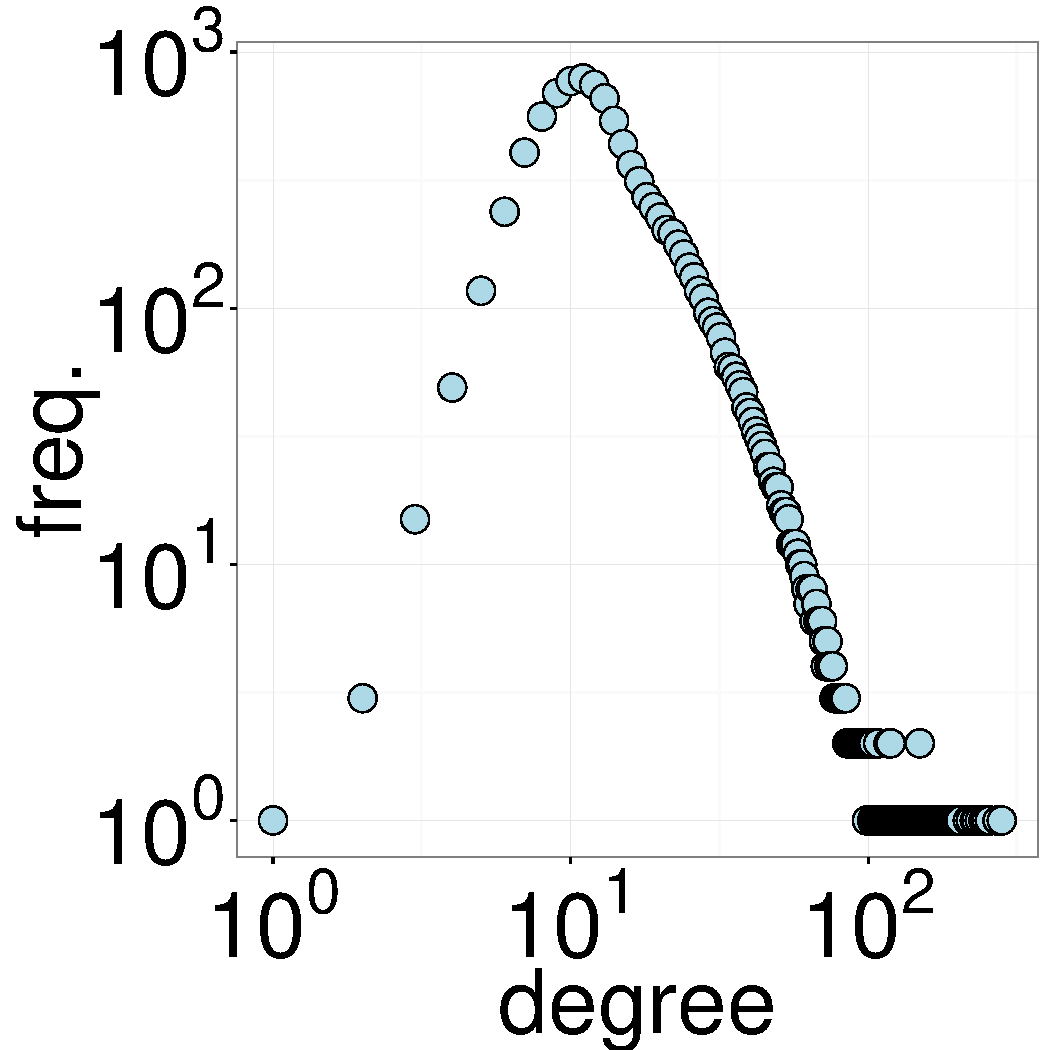
\includegraphics[width=2.5cm]{figures/distr_stupnu_Setting2}
    \caption{$Setting_2$}
		  \end{subfigure}
   \begin{subfigure}{2.7cm}
    \centering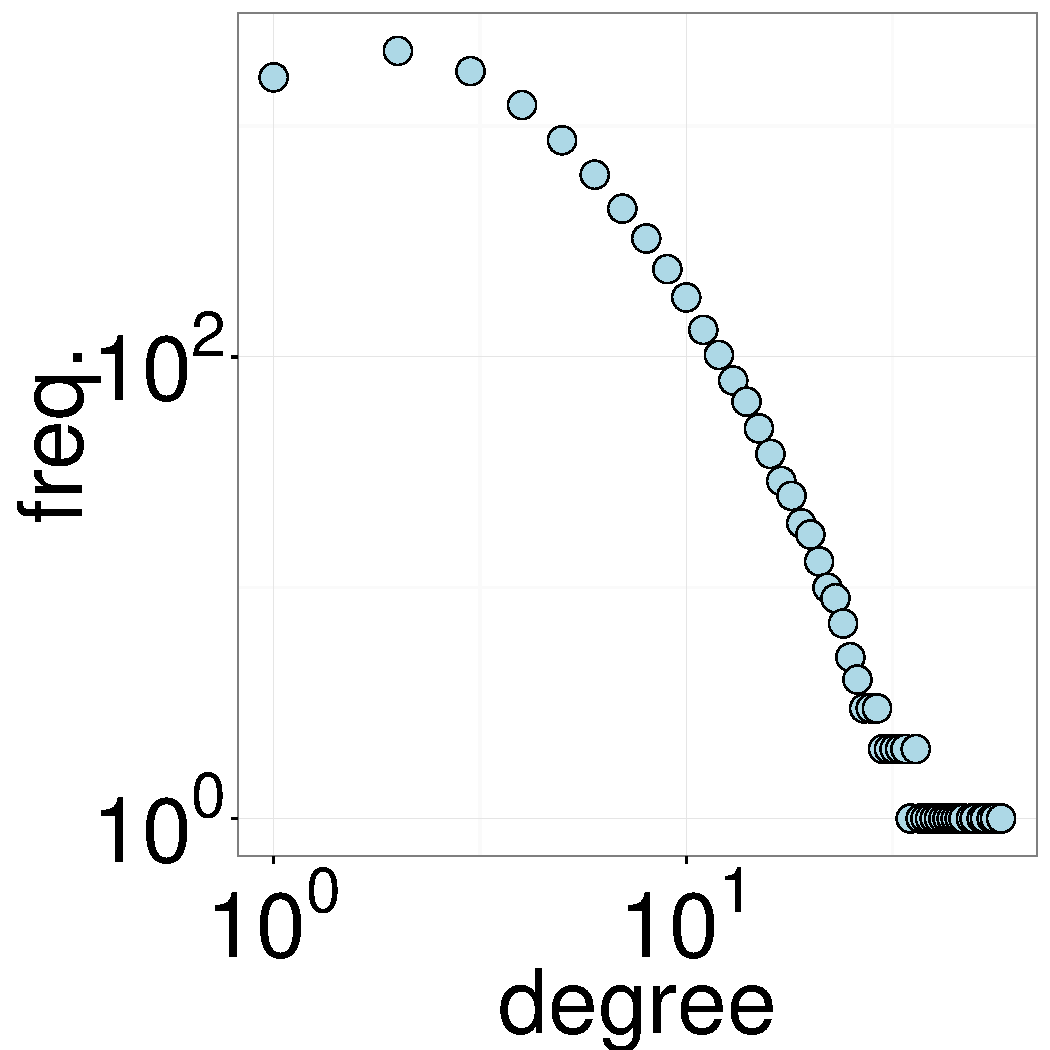
\includegraphics[width=2.5cm]{figures/distr_stupnu_Setting3}
    \caption{$Setting_3$}
  \end{subfigure}
	\caption{Degree distribution}
\label{fig:DD}
\end{figure}

\begin{figure}[ht]
	\centering
  \begin{subfigure}{2.7cm}
    \centering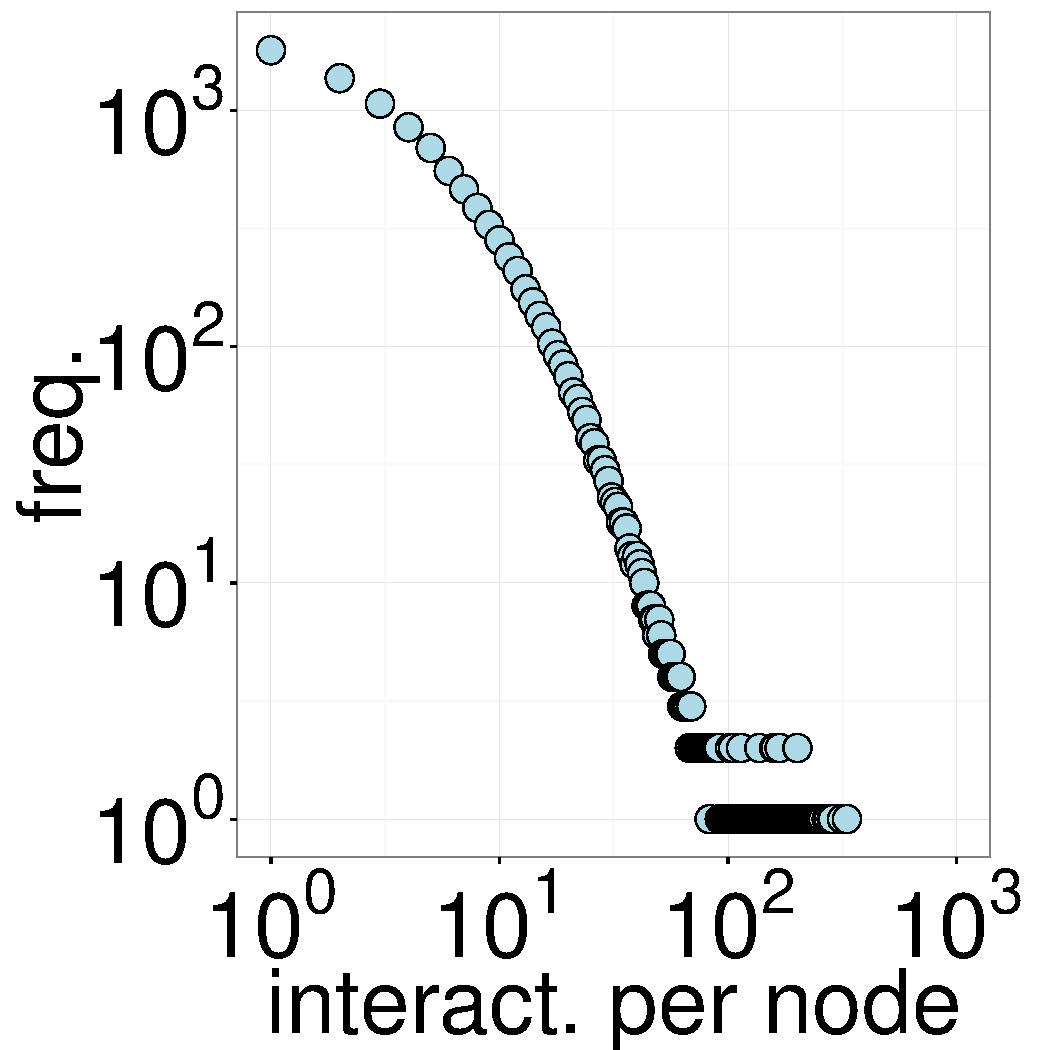
\includegraphics[width=2.5cm]{figures/inter_per_vert_Setting1}
    \caption{$Setting_1$}
  \end{subfigure}
  \begin{subfigure}{2.7cm}
    \centering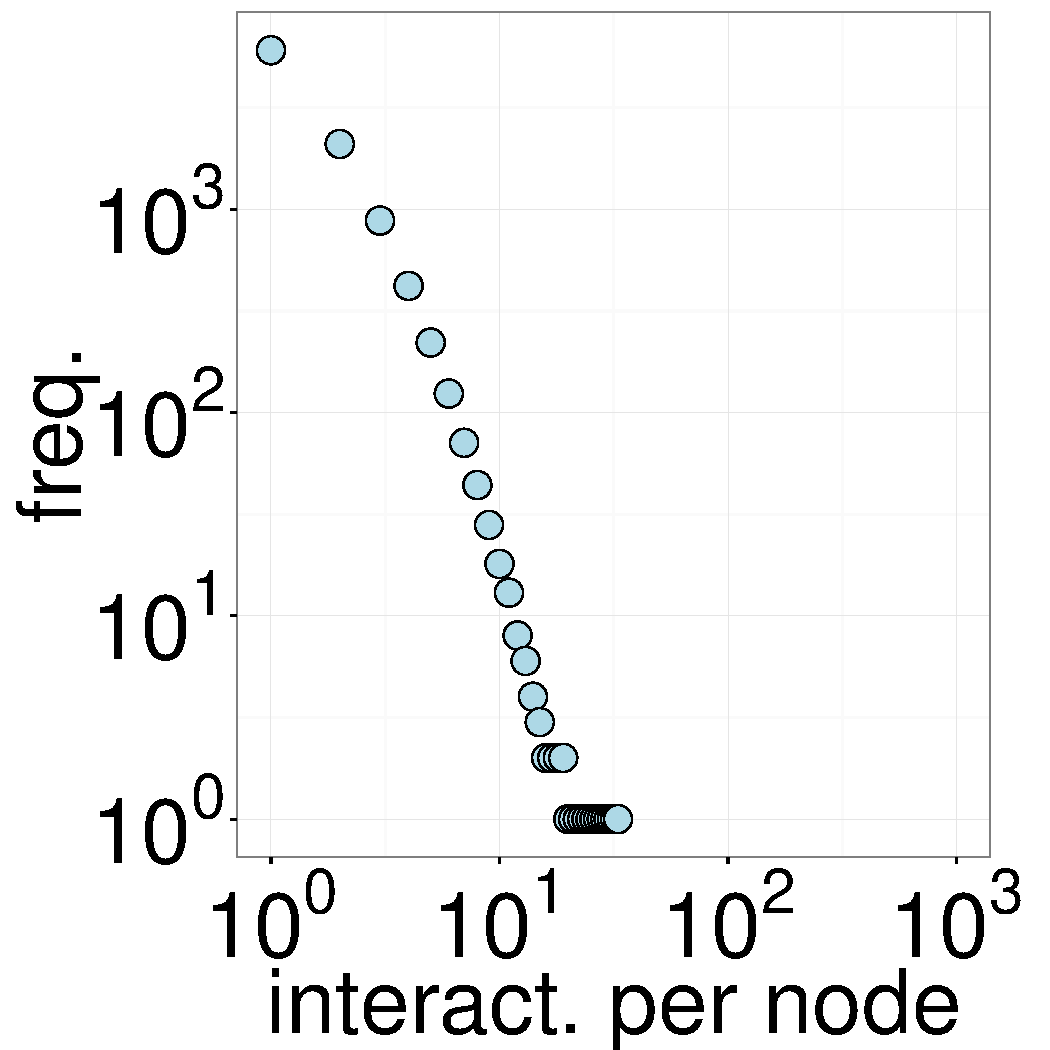
\includegraphics[width=2.5cm]{figures/inter_per_vert_Setting2}
    \caption{$Setting_2$}
		  \end{subfigure}
   \begin{subfigure}{2.7cm}
    \centering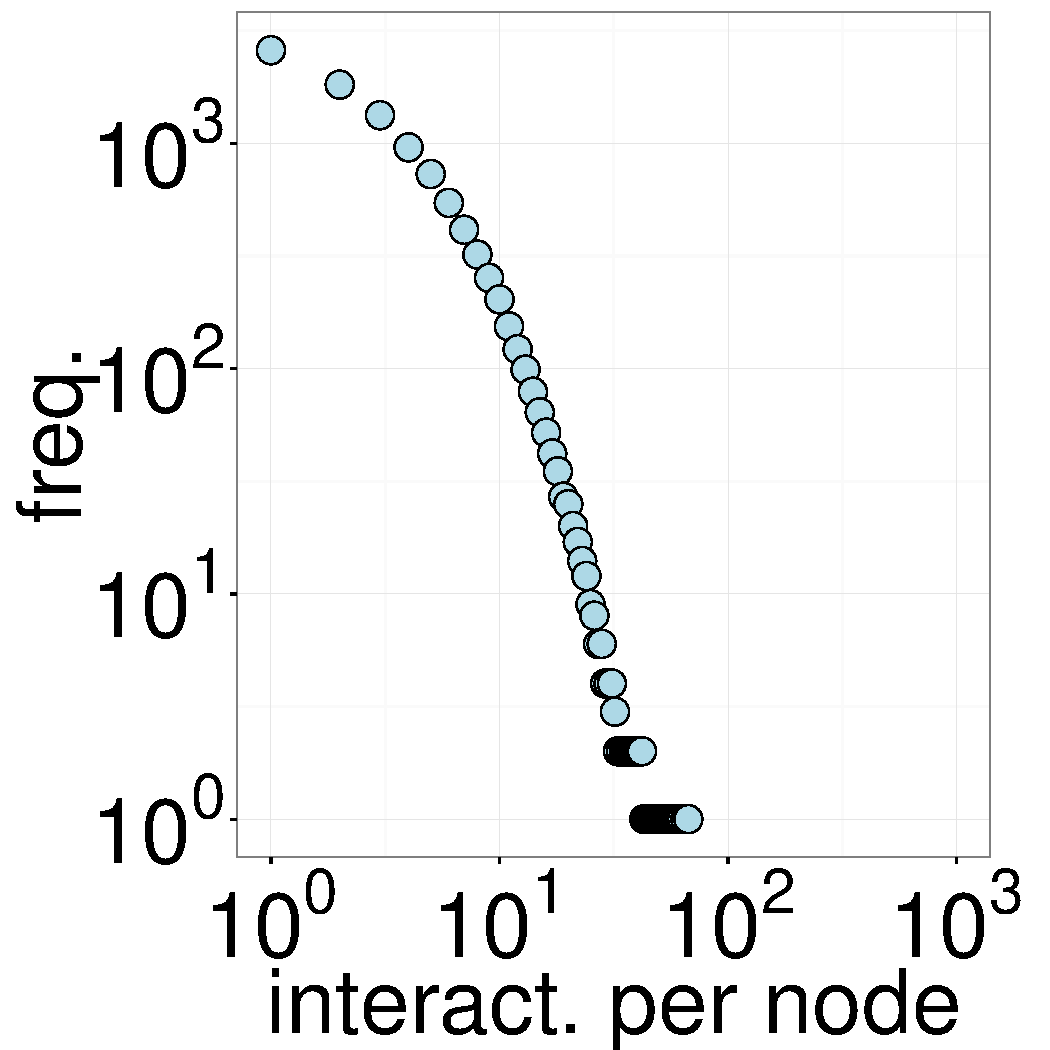
\includegraphics[width=2.5cm]{figures/inter_per_vert_Setting3}
    \caption{$Setting_3$}
  \end{subfigure}
	\caption{Interactions per	node}
\label{fig:IpN}
\end{figure}

\begin{figure}[ht]
	\centering
  \begin{subfigure}{2.7cm}
    \centering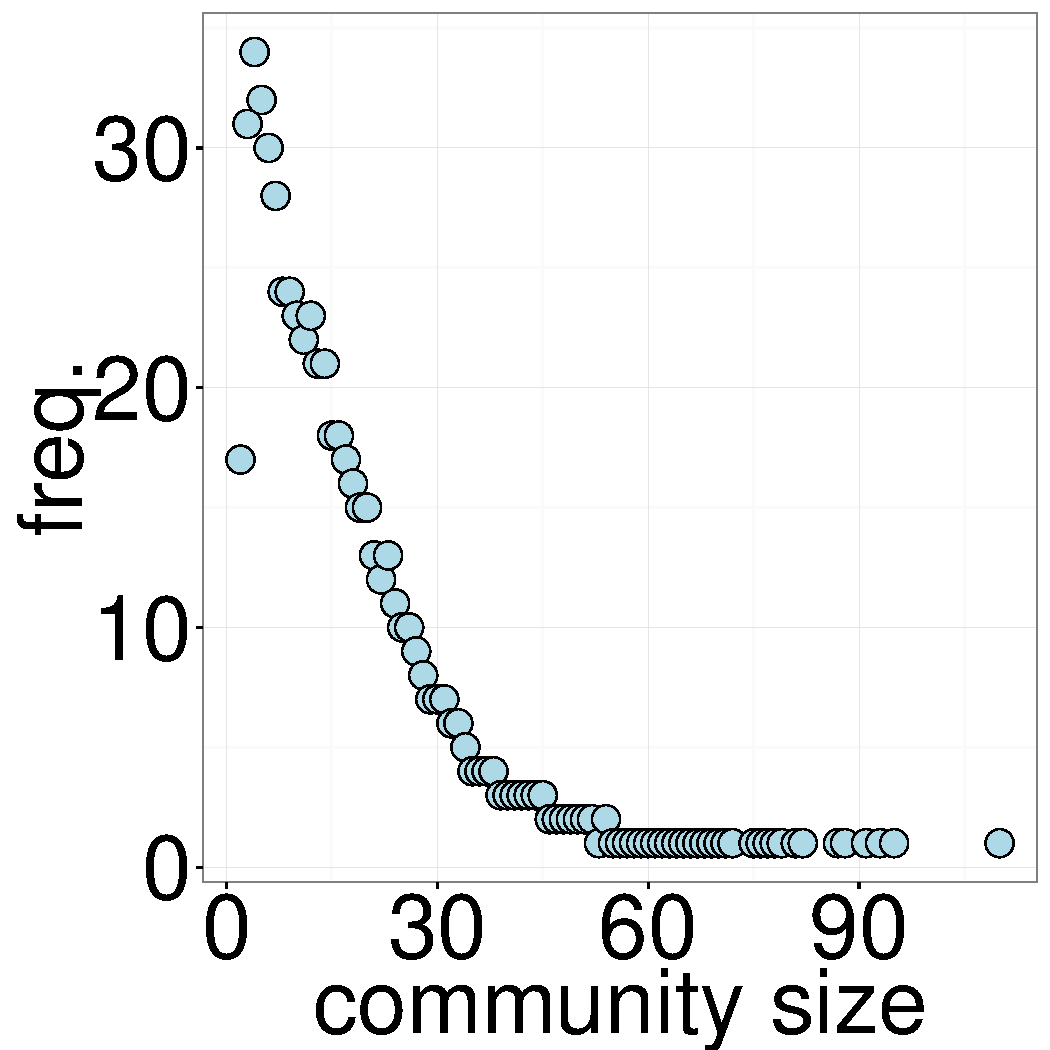
\includegraphics[width=2.5cm]{figures/dist_vel_komf_Setting1}
    \caption{$Setting_1$}
  \end{subfigure}
  \begin{subfigure}{2.7cm}
    \centering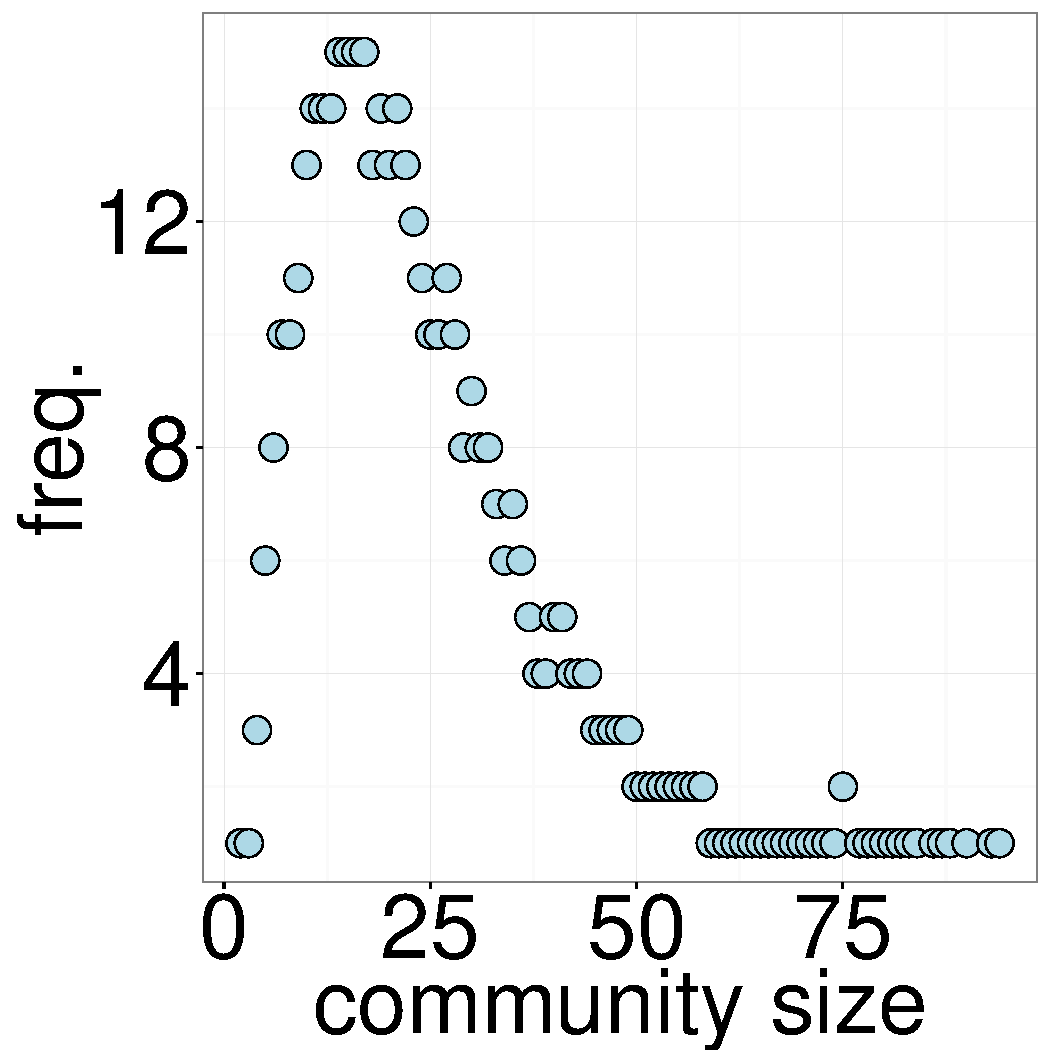
\includegraphics[width=2.5cm]{figures/dist_vel_komf_Setting2}
    \caption{$Setting_2$}
		  \end{subfigure}
   \begin{subfigure}{2.7cm}
    \centering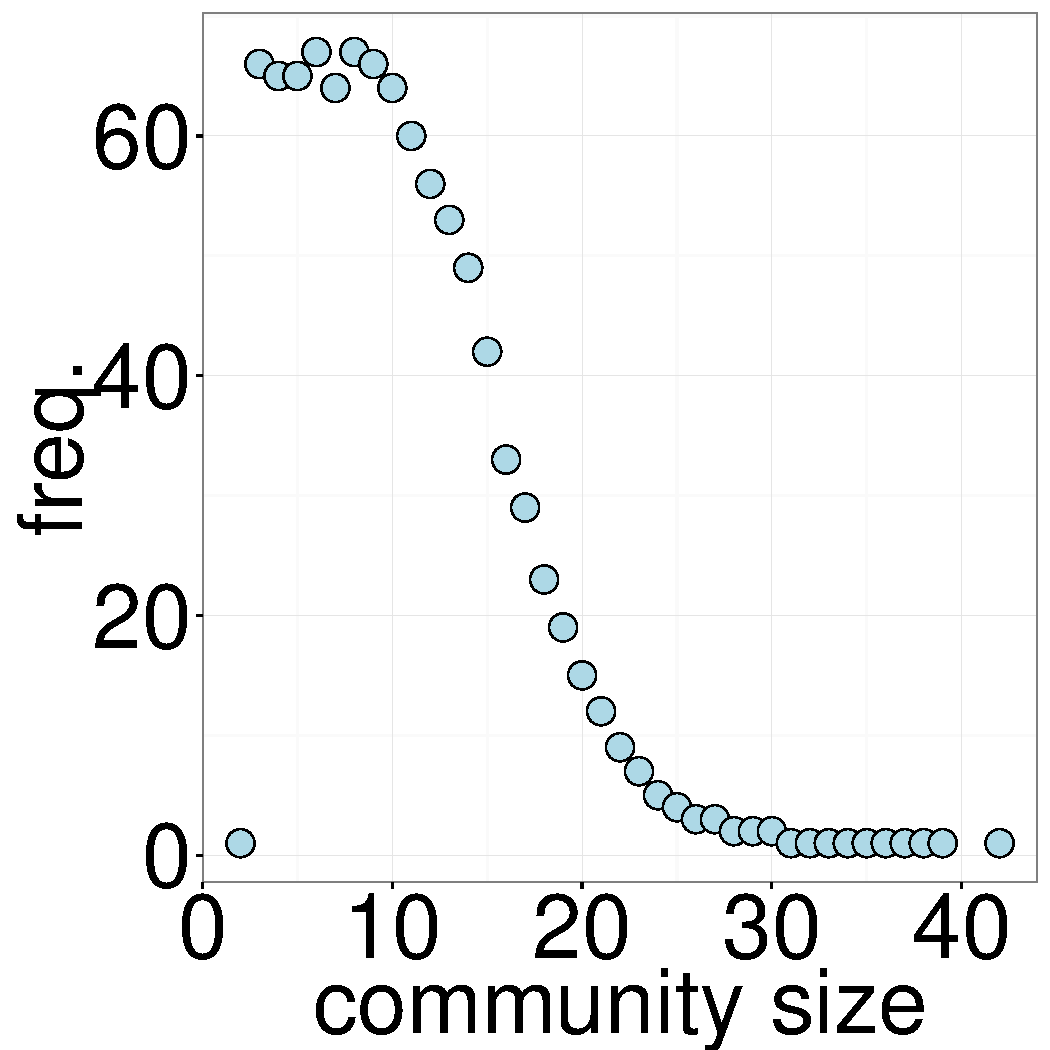
\includegraphics[width=2.5cm]{figures/dist_vel_komf_Setting3}
    \caption{$Setting_3$}
  \end{subfigure}
	\caption{Community size}
\label{fig:ComSize}
\end{figure}


\subsection{Properties of Generated Network}

\begin{table*}[ht]
  \centering
  \caption{Global properties}
		\begin{tabular}{|c|r|rrrrrrrrrrr|}
\hline
Setting &  & $n$ & $m$ & $<$k$>$ &  $<$l$>$ & $l_{max}$ & $CC$ & $r$ & $com_{IM}$ & $com_L$ & $Q_{IM}$ & $Q_L$ \\ 
\hline
$Setting_1$ & mean & 10001.10 & 40108.97 & 8.0209 & 4.8101 & 12.07 & 0.6555 & 0.14522 & 609.40 & 54.70 & 0.6424 & 0.7119 \\ 
& sd & 0.31 & 398.80 & 0.0797 & 0.0421 & 0.64 & 0.0029 & 0.01769 & 12.37 & 7.04 & 0.0062 & 0.0085 \\ 
\hline	
$Setting_2$ & mean & 10003.87 & 88620.40 & 17.7172 & 4.2369 & 8.43  & 0.8087 & 0.12961 & 422.60 & 42.90 & 0.6772 & 0.7334 \\ 
& sd & 1.53 & 797.95 & 0.1600 & 0.0277 & 0.63  & 0.0018 & 0.00913 & 10.30 & 2.78 & 0.0049 & 0.0067 \\ 
\hline
$Setting_3$ & mean & 10001.17 & 21494.57 & 4.2984 & 6.8965 & 16.23 & 0.4784 & 0.19907 & 953.30 & 68.70 & 0.7276 & 0.8129 \\ 
&  sd & 0.46 & 142.64 & 0.0285 & 0.0609 & 0.63 & 0.0044 & 0.01222 & 15.55 & 3.19 & 0.0035 & 0.0038 \\ 
\hline
\end{tabular}%
  \label{tab:gp}%
\end{table*}%
\begin{table}[ht]
  \centering
  \caption{Interactions}
\begin{tabular}{|r|r|rrr|}
	\hline
Setting & & $I$ & $<$i$>$ & $<$s$>$ \\ 
\hline
$Setting_1$ & mean & 28561.90 & 8.0887 & 2.8323 \\ 
&  sd & 278.93 & 0.0817 & 0.0082 \\ 
\hline	
$Setting_2$ & mean & 1664.53 & 1.8278 & 10.9860 \\ 
& sd & 17.69 & 0.0115 & 0.0824 \\
\hline	
$Setting_3$ & mean & 22204.43 & 4.3772 & 1.9716 \\ 
& sd & 202.06 & 0.0292 & 0.0069 \\ 
\hline
	\end{tabular}%
  \label{tab:interact}%
\end{table}%

In the first experiment, we show the properties of networks generated with different settings. We generated for each setting $100$ networks with approximately $10000$ nodes. Table \ref{tab:gp} summarizes average values (and standard deviation) of measured properties for each setting. Measured properties include number of nodes $n$ and edges $m$, average degree $<$k$>$, average shortest path length $<$l$>$, diameter $L_{max}$, average clustering coefficient $CC$, assortativity $r$, number of communities detected by Infomap \cite{rosvall2009map} $com_{IM}$ and Louvain \cite{blondel2008fast} $com_L$ algorithm, and corresponding modularities $Q_{IM}$ and $Q_L$, respectively. Table \ref{tab:interact} contains average values associated with the temporality of the network, i.e. total number of interactions $I$, average number of interactions $<$i$>$ and average number of nodes in interaction $<$s$>$. Figures \ref{fig:DD}-\ref{fig:ComSize} show degree distribution, number of interactions distribution and distributions of community size detected by Infomap algorithm.

The experiment indicates that all three settings generate networks with small-world and scale-free characteristics. The first and second setting have generated networks of high average clustering coefficient. Networks have a tendency to be assortative. Assortativity values correspond to all settings to the values known from social networks \cite{newman2002assortative}. Generated networks also have community structure and a high modularity for all settings.

\begin{figure}[ht]
\centering
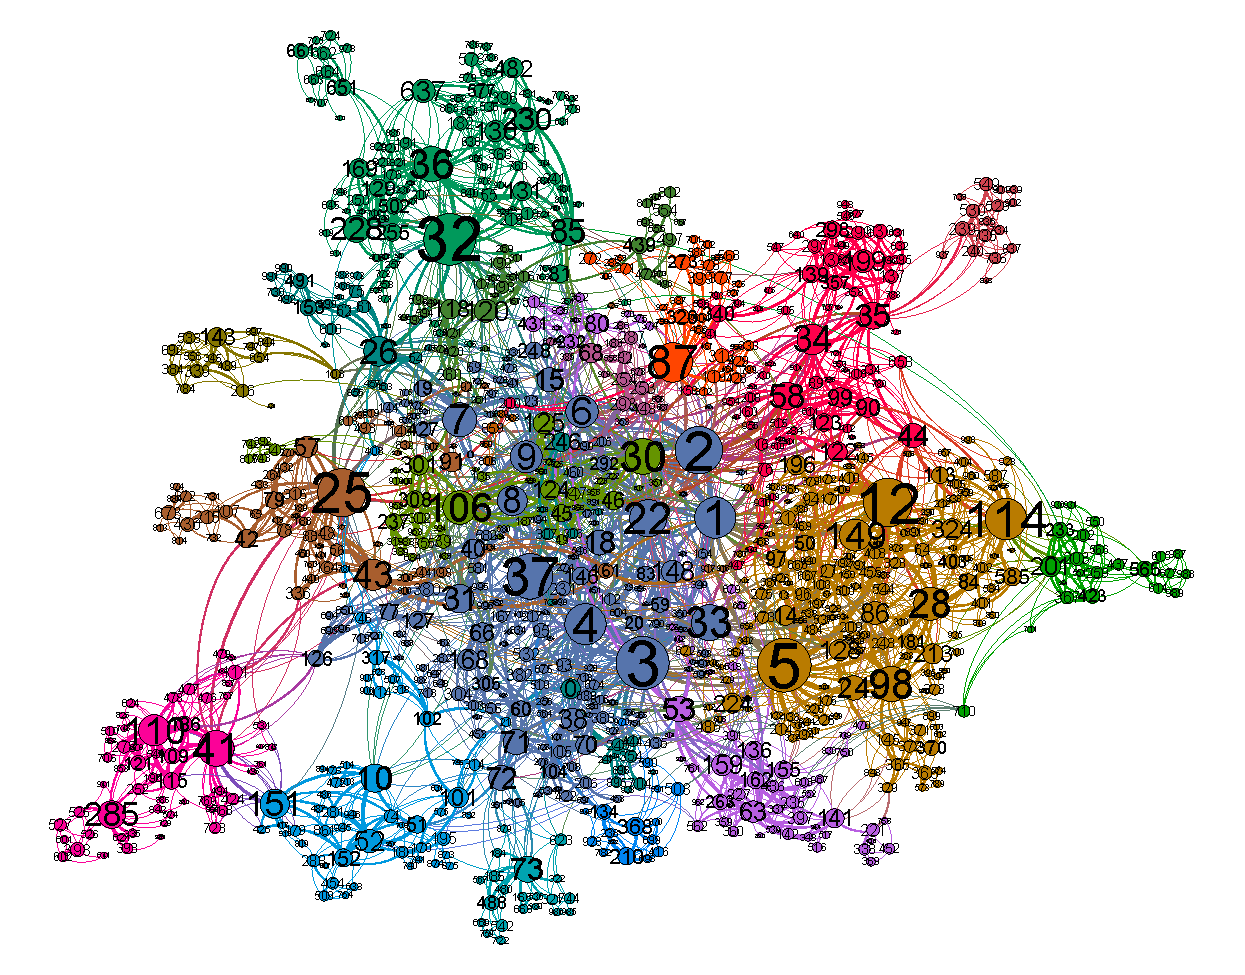
\includegraphics[width=\linewidth]{figures/setting1_1000}
  \caption{Network: 1000 nodes, $Setting_1$}
	\label{fig:Set1000}
\end{figure}

Figure \ref{fig:Set1000} shows a network with $1000$ nodes and $3599$ edges generated with $Setting_1$. A total of $2830$ interactions took place. The size of nodes and strength of edges correspond to the number of interactions they took part in, the labels indicate the order in which nodes were created. The network has an overlapping community and core-periphery structure. Colored 19 communities were detected by Louvain method, modularity is $0.746$.

\subsection{Evolution of Generated Network}
The subject of the second experiment is one network generated with $Setting_1$. The aim is to show the development of network properties during its growth. The values for each characteristic are measured when the network has $10, 20, 50, 100$, ..., and $10000$ nodes. The results are summarized in Table \ref{tab:Evolut}.

\begin{table*}[ht]
  \centering
  \caption{Evolution of network properties}
	\begin{tabular}{|r|rrrrrrrrrr|}

\hline
  $n$ & $m$ & $<$k$>$ &  $<$l$>$ & $l_{max}$ & $CC$ & $r$ & $com_{IM}$ & $com_L$ & $Q_{IM}$ & $Q_L$ \\
\hline
  10 & 27.00 & 5.4000 & 1.4000 & 20 & 0.8195 & -0.41738 & 1 & 3 & 0.0000 & 0.0590 \\ 
 20 & 53.00 & 5.3000 & 2.0684 & 5 & 0.5804 & -0.09355 & 2 & 4 & 0.0361 & 0.2398 \\ 
  50 & 184.00 & 7.3600 & 2.5004 & 7 & 0.6248 & -0.00886 & 5 & 5 & 0.2957 & 0.3742 \\ 
100 & 388.00 & 7.7600 & 2.8731 & 6 & 0.6793 & 0.09177 & 11 & 9 & 0.4259 & 0.4613 \\ 
 200 & 812.00 & 8.1200 & 3.1859 & 7 & 0.6824 & 0.05107 & 20 & 11 & 0.5002 & 0.5121 \\ 
500 & 2112.00 & 8.4480 & 3.6095 & 8 & 0.6394 & 0.11911 & 44 & 11 & 0.5540 & 0.5849 \\ 
 1000 & 4053.00 & 8.1060 & 3.9402 & 9 & 0.6592 & 0.14528 & 83 & 17 & 0.5812 & 0.6341 \\ 
2000 & 8306.00 & 8.3060 & 4.2054 & 10 & 0.6538 & 0.14016 & 151 & 24 & 0.5972 & 0.6714 \\ 
5000 & 20316.00 & 8.1264 & 4.5344 & 12 & 0.6603 & 0.15823 & 342 & 44 & 0.6203 & 0.6827 \\ 
10000 & 40476.00 & 8.0952 & 4.8015 & 11 & 0.6557 & 0.15351 & 645 & 64 & 0.6307 & 0.7003 \\ 
\hline
  \end{tabular}
	  \label{tab:Evolut}%
\end{table*}%
	
Figure \ref{fig:EvolNet}, similarly to the previous experiment, shows the distribution of degree, number of interactions and size of communities. The evolution of these properties is portrayed when network has $100, 200, 1000, 5000, 10000$ nodes.

\begin{figure*}[ht]
\centering
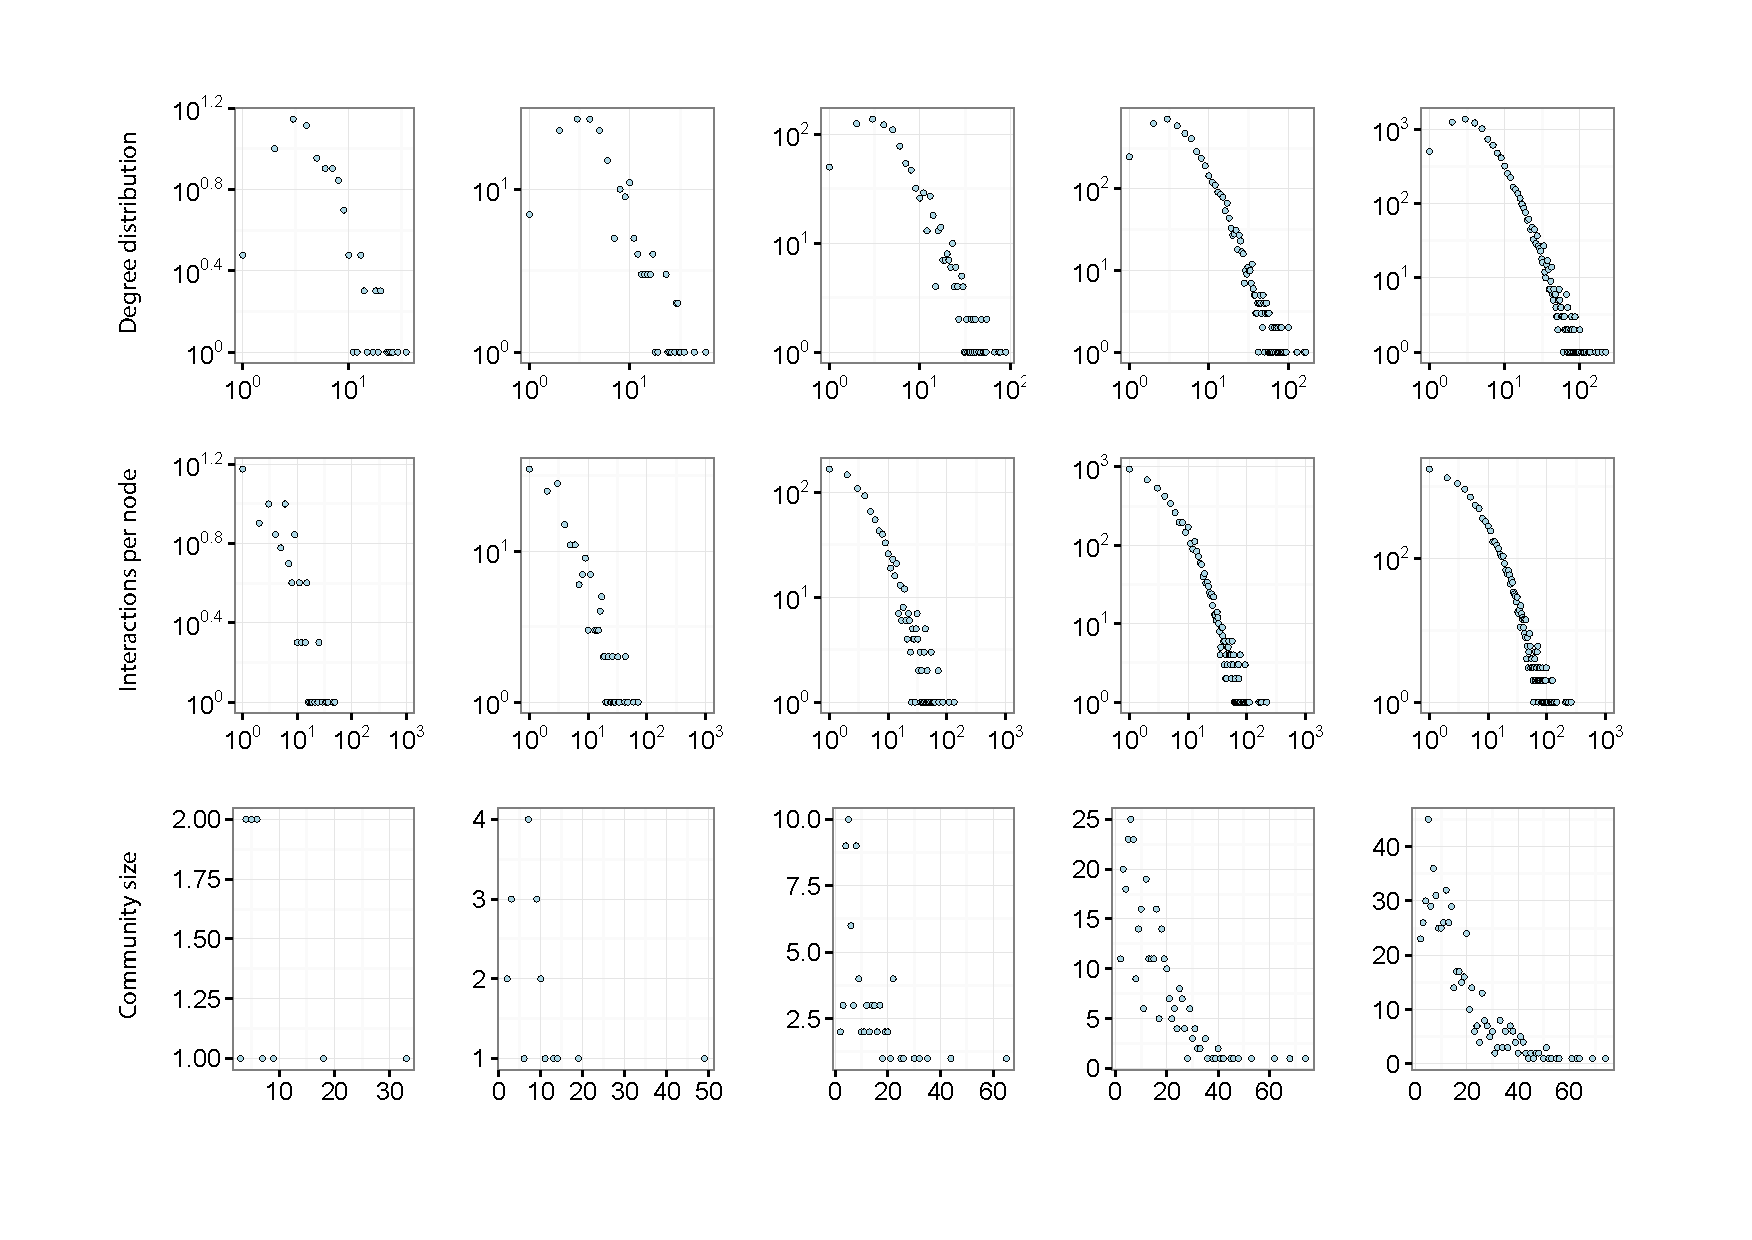
\includegraphics[width=46em]{figures/distribution_10_20_50}
\caption{Evolution of network (100, 200, 1000, 5000, 10000 nodes)}
\label{fig:EvolNet}
\end{figure*}

Key properties (average degree, shortest path, clustering coefficient, assortativity, modularity) happen to stabilize their values between $1000$ and $10000$ nodes. Our experiments show that  generated networks with other settings also have similar behavior. Figure \ref{fig:InterEvol} shows the evolution of the number of interactions for fifteen nodes with the highest number of interactions at the end of the generation process. The ID of a node represents the moment of its creation. The trend shows how the chances of participating in interactions increase for nodes that already have a high number of interactions.

\begin{figure}[ht]
\centering
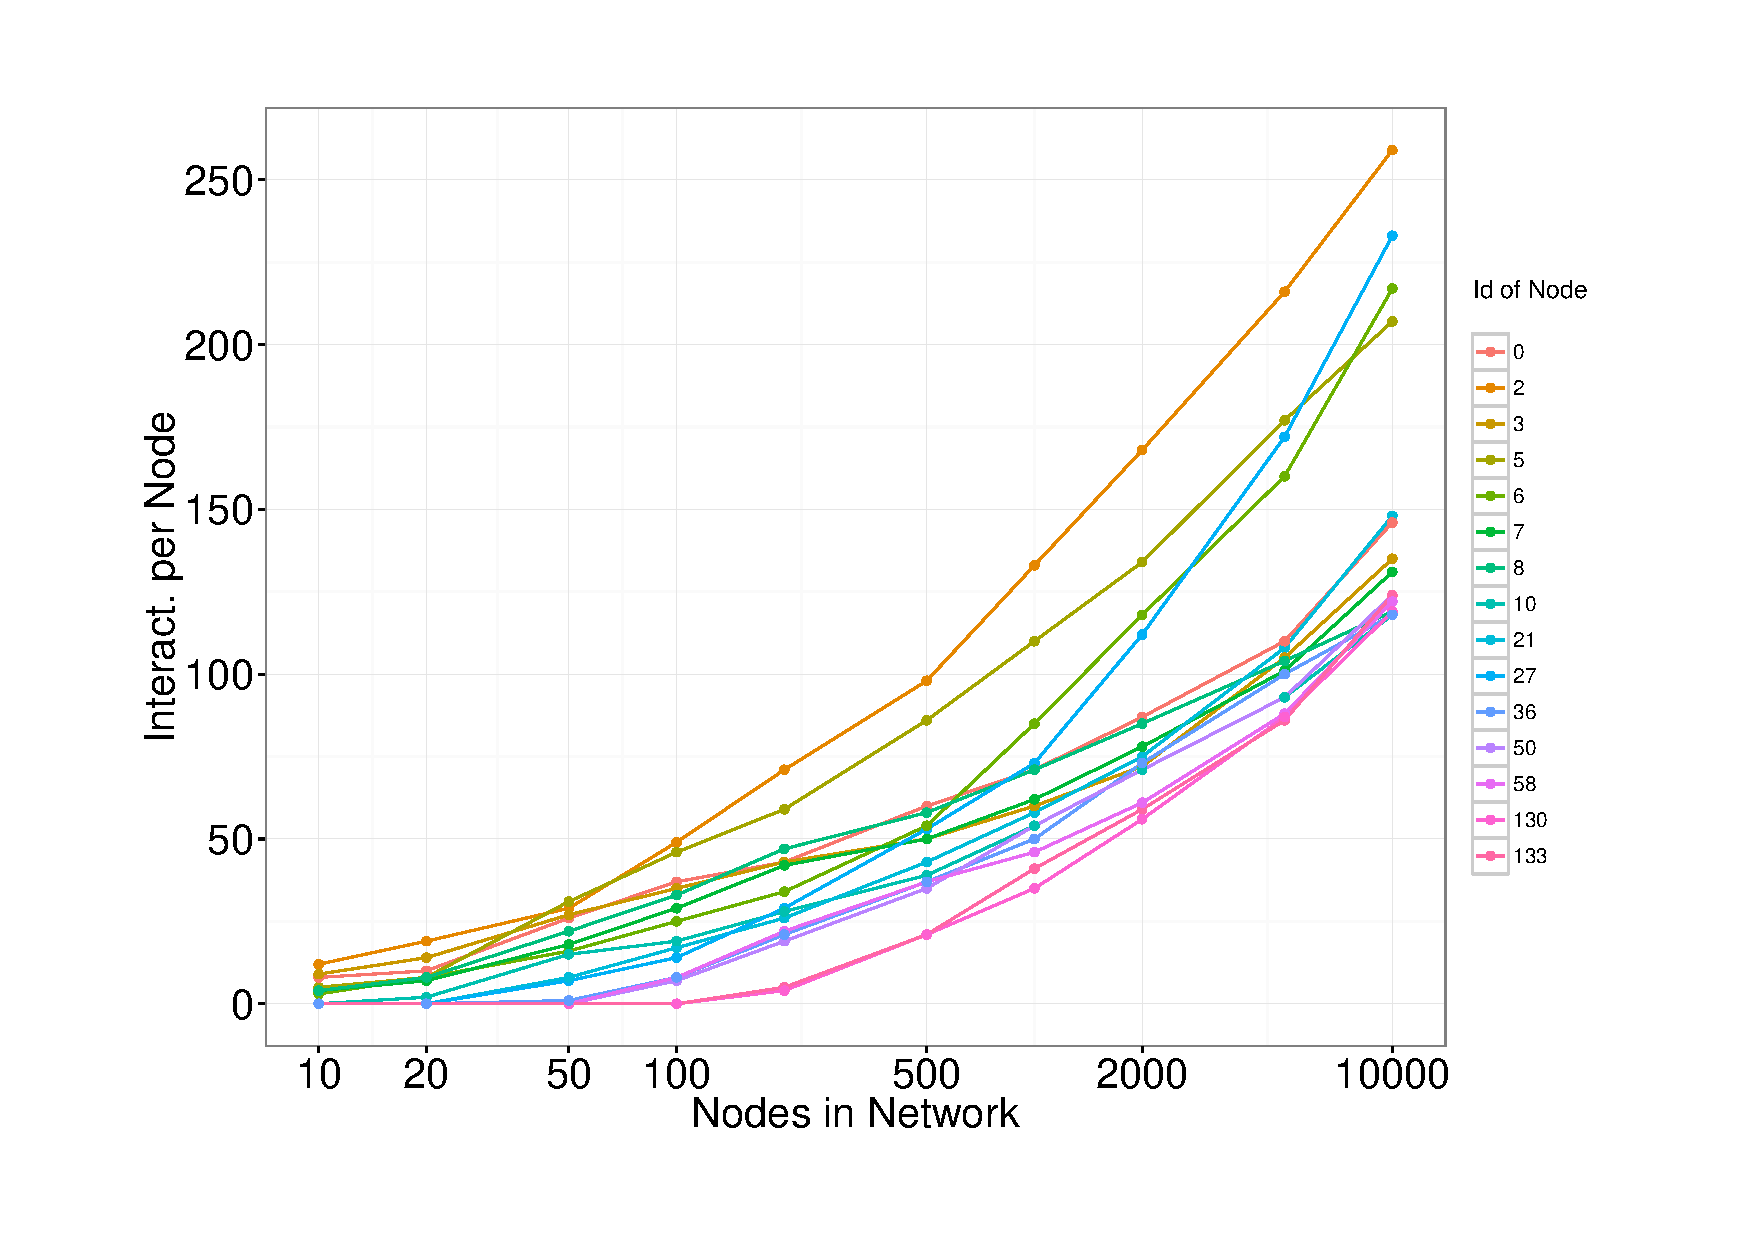
\includegraphics[width =\linewidth]{figures/Interaction_evolution}
\caption{Evolution of nodes with the most interactions}
\label{fig:InterEvol}
\end{figure}


\subsection{Correlations}
In this experiment, we compare the analyzed real-world network with generated networks. For each setting we generated a network with one million nodes. Then we examined the correlation between the node's creation time and it's degree and number of interactions, respectively. The emergence of the node is represented by its $ID$, which is in the order of its creation. Furthermore, we calculated the correlation between degree and number of node's interactions. We did the same for the analyzed DBLP dataset, where the order of nodes is to be understood as an estimate based on data pre-processing described in Section \ref{sec:dblp}.

\begin{table}[ht]
  \centering
  \caption{Correlations}
\begin{tabular}{|r|rrr|}
	\hline
Setting & $\rho(Id, k)$ & $\rho(Id, i)$ & $\rho(k, i)$ \\ 
\hline
$Setting_1$ & -0.59 & -0.50 & 0.96 \\  
\hline	
$Setting_2$ & -0.47 & -0.47 & 0.95 \\ 
\hline	
$Setting_3$ & -0.70 & -0.58 & 0.87 \\ 
\hline
DBLP & -0.23 & -0.18 & 0.84 \\ 
\hline
	\end{tabular}%
  \label{tab:corr}%
\end{table}%

The results summarized in Table \ref{tab:corr} show that regardless of the setting, the first two correlations are much higher in the 3-lambda model than in the DBLP dataset (Pearson's correlation coefficient was used). Thus, in the presented model, older nodes have a higher (and continuous) chance to participate in interactions than in reality. The cause is probably the aging of nodes in real-world networks where nodes, at different times, no longer participate in interactions. This significantly affects the evolution (growth) and some properties of the network.

Previous experiments demonstrated that despite the absence of aging, generated networks have very good properties. We have not, therefore, for reasons of simplicity, incorporated any of the known models of aging (e.g. inspired by \cite{dorogovtsev2000evolution, xu2010evolutionary}) to the 3-lambda network model.

\section{Conclusion}
\label{sec:conclusion}

This paper presents a matrix factorization based approach to text
outlier analysis. The approach is designed to adjust well to the
widely varying structures in different localities of the data, and
therefore provides more robust methods than competing models. The
approach has the potential to be applied to other domains with
similar structure, and as a specific example, we provide experiments
on market  basket data. We also presented extensive experimental
results, which illustrate the superiority of the approach.  
Our code can be downloaded from 
\url{https://github.com/ramkikannan/outliernmf} and 
tried with any text dataset. 

In this paper, we had a parallel implementation using the
Matlab's parallel computing toolbox to run in multicore environments.
In the future, we would like to explore a scalable implementation
of our algorithm. The solution is embarrassingly parallelizable,
and would like to experiment in web scale data. One of the potential
extension is incorporating temporal and spatial aspects into the model.
Such an extension, make the solution applicable to emerging 
applications such as topic detection and streaming data. 
%In the recent times,
%approximate matrix factorization techniques are explored by
%randomly sampling the input matrix. We can reduce the computation
%time for very large matrices using such sampling techniques. We would like
%to explore a sampling based solution for our model. 
We experimented
the solution primarily on text data and market basket data. In future
work, we will extend this broader approach to other domains such as
video data.


The authors would like to thank Duane Merrill for his valuable comments on CUB and our paper drafts.
Also, thanks to NVIDIA for providing the GPUs that made this research possible.
We appreciate the funding support from UC Lab Fees Research Program Award 12-LR-238449, DFG grant ME 2088/3-1, MADALGO (Center for Massive Data Algorithmics), NSF awards CCF-1017399 and OCI-1032859, Sandia LDRD award \#13-0144, and a 2016--17 NVIDIA Graduate Fellowship.


\bibliographystyle{abbrv}
\bibliography{references}

\end{document}
